\documentclass{book}
\usepackage[a4paper,top=2.5cm,bottom=2.5cm,left=2.5cm,right=2.5cm]{geometry}
\usepackage{makeidx}
\usepackage{natbib}
\usepackage{graphicx}
\usepackage{multicol}
\usepackage{float}
\usepackage{listings}
\usepackage{color}
\usepackage{ifthen}
\usepackage[table]{xcolor}
\usepackage{textcomp}
\usepackage{alltt}
\usepackage{ifpdf}
\ifpdf
\usepackage[pdftex,
            pagebackref=true,
            colorlinks=true,
            linkcolor=blue,
            unicode
           ]{hyperref}
\else
\usepackage[ps2pdf,
            pagebackref=true,
            colorlinks=true,
            linkcolor=blue,
            unicode
           ]{hyperref}
\usepackage{pspicture}
\fi
\usepackage[utf8]{inputenc}
\usepackage{mathptmx}
\usepackage[scaled=.90]{helvet}
\usepackage{courier}
\usepackage{sectsty}
\usepackage{amssymb}
\usepackage[titles]{tocloft}
\usepackage{doxygen}
\lstset{language=C++,inputencoding=utf8,basicstyle=\footnotesize,breaklines=true,breakatwhitespace=true,tabsize=8,numbers=left }
\makeindex
\setcounter{tocdepth}{3}
\renewcommand{\footrulewidth}{0.4pt}
\renewcommand{\familydefault}{\sfdefault}
\hfuzz=15pt
\setlength{\emergencystretch}{15pt}
\hbadness=750
\tolerance=750
\begin{document}
\hypersetup{pageanchor=false,citecolor=blue}
\begin{titlepage}
\vspace*{7cm}
\begin{center}
{\Large Alive \\[1ex]\large 1.\-0 }\\
\vspace*{1cm}
{\large Generated by Doxygen 1.8.3.1}\\
\vspace*{0.5cm}
{\small Tue Apr 30 2013 15:22:24}\\
\end{center}
\end{titlepage}
\clearemptydoublepage
\pagenumbering{roman}
\tableofcontents
\clearemptydoublepage
\pagenumbering{arabic}
\hypersetup{pageanchor=true,citecolor=blue}
\chapter{Alive Documentation}
\label{index}\hypertarget{index}{}Below is a brief overview of and guide to the classes and their relations. If you are new to \hyperlink{classQCustomPlot}{Q\-Custom\-Plot} and just want to start using it, it's recommended to look at the examples/tutorials at

\href{http://www.WorksLikeClockWork.com/index.php/components/qt-plotting-widget}{\tt http\-://www.\-Works\-Like\-Clock\-Work.\-com/index.\-php/components/qt-\/plotting-\/widget}

This documentation is especially helpful when you're familiar with the basic concept of how to use Q\-Custom\-Plot and you wish to learn more about specific functionality.\hypertarget{index_simpleoverview}{}\section{Simplified Class Overview}\label{index_simpleoverview}

\begin{DoxyImageNoCaption}
  \mbox{\includegraphics[width=1.2\textwidth]{ClassesOverviewSimplified.png}}
\end{DoxyImageNoCaption}
  \begin{center}Simplified diagram of most important classes, view the \hyperlink{classoverview}{Class Overview} to see a full overview.\end{center} 

The central widget which displays the plottables and axes on its surface is \hyperlink{classQCustomPlot}{Q\-Custom\-Plot}. Usually, you don't create the axes yourself, but you use the ones already inside every \hyperlink{classQCustomPlot}{Q\-Custom\-Plot} instance (x\-Axis, y\-Axis, x\-Axis2, y\-Axis2).\hypertarget{index_plottables}{}\section{Plottables}\label{index_plottables}
{\itshape Plottables} are classes that display any kind of data inside the \hyperlink{classQCustomPlot}{Q\-Custom\-Plot}. They all derive from \hyperlink{classQCPAbstractPlottable}{Q\-C\-P\-Abstract\-Plottable}. For example, the \hyperlink{classQCPGraph}{Q\-C\-P\-Graph} class is a plottable that displays a graph inside the plot with different line styles, scatter styles, filling etc.

Since plotting graphs is such a dominant use case, \hyperlink{classQCustomPlot}{Q\-Custom\-Plot} has a special interface for working with \hyperlink{classQCPGraph}{Q\-C\-P\-Graph} plottables, that makes it very easy to handle them\-:\par
 You create a new graph with \hyperlink{classQCustomPlot_a6fb2873d35a8a8089842d81a70a54167}{Q\-Custom\-Plot\-::add\-Graph} and access them with \hyperlink{classQCustomPlot_a6d3ed93c2bf46ab7fa670d66be4cddaf}{Q\-Custom\-Plot\-::graph}.

For all other plottables, you need to use the normal plottable interface\-:\par
 First, you create an instance of the plottable you want, e.\-g. 
\begin{DoxyCode}
\hyperlink{classQCPCurve}{QCPCurve} *newCurve = \textcolor{keyword}{new} \hyperlink{classQCPCurve}{QCPCurve}(customPlot->xAxis, customPlot->yAxis);
\end{DoxyCode}
 add it to the custom\-Plot with \hyperlink{classQCustomPlot_ab7ad9174f701f9c6f64e378df77927a6}{Q\-Custom\-Plot\-::add\-Plottable}\-: 
\begin{DoxyCode}
customPlot->addPlottable(newCurve);
\end{DoxyCode}
 and then modify the properties of the newly created plottable via {\ttfamily new\-Curve}.

Plottables (including graphs) can be retrieved via \hyperlink{classQCustomPlot_a32de81ff53e263e785b83b52ecd99d6f}{Q\-Custom\-Plot\-::plottable}. Since the return type of that function is the abstract base class of all plottables, \hyperlink{classQCPAbstractPlottable}{Q\-C\-P\-Abstract\-Plottable}, you will probably want to qobject\-\_\-cast (or dynamic\-\_\-cast) the returned pointer to the respective plottable subclass. (As usual, if the cast returns zero, the plottable wasn't of that specific subclass.)

All further interfacing with plottables (e.\-g how to set data) is specific to the plottable type. See the documentations of the subclasses\-: \hyperlink{classQCPGraph}{Q\-C\-P\-Graph}, \hyperlink{classQCPCurve}{Q\-C\-P\-Curve}, \hyperlink{classQCPBars}{Q\-C\-P\-Bars}, \hyperlink{classQCPStatisticalBox}{Q\-C\-P\-Statistical\-Box}.\hypertarget{index_axes}{}\section{Controlling the Axes}\label{index_axes}
As mentioned, \hyperlink{classQCustomPlot}{Q\-Custom\-Plot} has four axes by default\-: {\itshape x\-Axis} (bottom), {\itshape y\-Axis} (left), {\itshape x\-Axis2} (top), {\itshape y\-Axis2} (right).

Their range is handled by the simple \hyperlink{classQCPRange}{Q\-C\-P\-Range} class. You can set the range with the \hyperlink{classQCPAxis_a57d6ee9e9009fe88cb19db476ec70bca}{Q\-C\-P\-Axis\-::set\-Range} function. By default, the axes represent a linear scale. To set a logarithmic scale, set \hyperlink{classQCPAxis_adb6c5c45bdf899ea221881dd3b43b406}{Q\-C\-P\-Axis\-::set\-Scale\-Type} to \hyperlink{classQCPAxis_a36d8e8658dbaa179bf2aeb973db2d6f0abf5b785ad976618816dc6f79b73216d4}{Q\-C\-P\-Axis\-::st\-Logarithmic}. The logarithm base can be set freely with \hyperlink{classQCPAxis_a726186054be90487885a748aa1b42188}{Q\-C\-P\-Axis\-::set\-Scale\-Log\-Base}.

By default, an axis automatically creates and labels ticks in a sensible manner, i.\-e. with a tick interval that's pleasing to the viewer. See the following functions for tick manipulation\-:\par
 \hyperlink{classQCPAxis_ac891409315bc379e3b1abdb162c1a011}{Q\-C\-P\-Axis\-::set\-Ticks}, \hyperlink{classQCPAxis_ae867c23d3a6a7bd4d09cc66c5d018f63}{Q\-C\-P\-Axis\-::set\-Auto\-Ticks}, \hyperlink{classQCPAxis_a7c7111cbeac9ec5fcb40f93a1ef51a0b}{Q\-C\-P\-Axis\-::set\-Auto\-Tick\-Count}, \hyperlink{classQCPAxis_a99fe77b034e06f5b723995beab96e741}{Q\-C\-P\-Axis\-::set\-Auto\-Tick\-Step}, \hyperlink{classQCPAxis_a04ba16e1f6f78d70f938519576ed32c8}{Q\-C\-P\-Axis\-::set\-Tick\-Labels}, \hyperlink{classQCPAxis_a54f24f5ce8feea25209388a863d7e448}{Q\-C\-P\-Axis\-::set\-Tick\-Label\-Type}, \hyperlink{classQCPAxis_a1bddd4413df8a576b7ad4b067fb33375}{Q\-C\-P\-Axis\-::set\-Tick\-Label\-Rotation}, \hyperlink{classQCPAxis_af727db0acc6492c4c774c0700e738205}{Q\-C\-P\-Axis\-::set\-Tick\-Step}, \hyperlink{classQCPAxis_a62ec40bebe3540e9c1479a8fd2be3b0d}{Q\-C\-P\-Axis\-::set\-Tick\-Length},...

Each axis can be given an axis label (e.\-g. \char`\"{}\-Voltage \mbox{[}m\-V\mbox{]}\char`\"{}) with \hyperlink{classQCPAxis_a33bcc382c111c9f31bb0687352a2dea4}{Q\-C\-P\-Axis\-::set\-Label}.

The distance of an axis backbone to the respective \hyperlink{classQCustomPlot}{Q\-Custom\-Plot} widget border is called its margin. Normally, the margins are calculated automatically. To change this, set \hyperlink{classQCustomPlot_aed5bb30c9b04c1d0103ab8ef7190f23a}{Q\-Custom\-Plot\-::set\-Auto\-Margin} to false and set the margins manually with \hyperlink{classQCustomPlot_a990cbcb1da0cc93ebb06ceea7366c129}{Q\-Custom\-Plot\-::set\-Margin}.\hypertarget{index_legend}{}\section{Plot Legend}\label{index_legend}
Every \hyperlink{classQCustomPlot}{Q\-Custom\-Plot} owns a \hyperlink{classQCPLegend}{Q\-C\-P\-Legend} (as {\itshape legend}). That's a small window inside the plot which lists the plottables with an icon of the plottable line/symbol and a description. The Description is retrieved from the plottable name (\hyperlink{classQCPAbstractPlottable_ab79c7ba76bc7fa89a4b3580e12149f1f}{Q\-C\-P\-Abstract\-Plottable\-::set\-Name}). Plottables can be added and removed from the legend via \hyperlink{classQCPAbstractPlottable_a70f8cabfd808f7d5204b9f18c45c13f5}{Q\-C\-P\-Abstract\-Plottable\-::add\-To\-Legend} and \hyperlink{classQCPAbstractPlottable_aa1f350e510326d012b9a9c9249736c83}{Q\-C\-P\-Abstract\-Plottable\-::remove\-From\-Legend}. By default, adding a plottable to \hyperlink{classQCustomPlot}{Q\-Custom\-Plot} automatically adds it to the legend, too. This behaviour can be modified with the \hyperlink{classQCustomPlot_ad8858410c2db47b7104040a3aa61c3fc}{Q\-Custom\-Plot\-::set\-Auto\-Add\-Plottable\-To\-Legend} property.

The \hyperlink{classQCPLegend}{Q\-C\-P\-Legend} provides an interface to access, add and remove legend items directly, too. See \hyperlink{classQCPLegend_a454272d7094437beb3278a2294006da5}{Q\-C\-P\-Legend\-::item}, \hyperlink{classQCPLegend_a5ee80cf83f65e3b6dd386942ee3cc1ee}{Q\-C\-P\-Legend\-::item\-With\-Plottable}, \hyperlink{classQCPLegend_a3ab274de52d2951faea45a6d975e6b3f}{Q\-C\-P\-Legend\-::add\-Item}, \hyperlink{classQCPLegend_ac91595c3eaa746fe6321d2eb952c63bb}{Q\-C\-P\-Legend\-::remove\-Item} for example.\hypertarget{index_userinteraction}{}\section{User Interactions}\label{index_userinteraction}
\hyperlink{classQCustomPlot}{Q\-Custom\-Plot} currently supports dragging axis ranges with the mouse (\hyperlink{classQCustomPlot_aa0e1c44295da2706d0f12ad48f64b806}{Q\-Custom\-Plot\-::set\-Range\-Drag}), zooming axis ranges with the mouse wheel (\hyperlink{classQCustomPlot_ad4a0919e471549a2daea517ce6538ad8}{Q\-Custom\-Plot\-::set\-Range\-Zoom}) and a complete selection mechanism of most objects.

The availability of these interactions is controlled with \hyperlink{classQCustomPlot_add9cc886ff5257f64fb4117cf6c135fe}{Q\-Custom\-Plot\-::set\-Interactions}. For details about the interaction system, see the documentation there.

Further, \hyperlink{classQCustomPlot}{Q\-Custom\-Plot} always emits corresponding signals, when objects are clicked or double\-Clicked. See \hyperlink{classQCustomPlot_a57e5efa8a854620e9bf62d31fc139f53}{Q\-Custom\-Plot\-::plottable\-Click}, \hyperlink{classQCustomPlot_af2e6f1cea923dae437681d01ce7d0c31}{Q\-Custom\-Plot\-::plottable\-Double\-Click} and \hyperlink{classQCustomPlot_abf635f8b56ab5c16d5de9f358543e82b}{Q\-Custom\-Plot\-::axis\-Click} for example.\hypertarget{index_items}{}\section{Items}\label{index_items}
Apart from plottables there is another category of plot objects that are important\-: Items. The base class of all items is \hyperlink{classQCPAbstractItem}{Q\-C\-P\-Abstract\-Item}. An item sets itself apart from plottables in that it's not necessarily bound to any axes. This means it may also be positioned in absolute pixel coordinates or placed at a relative position on the axis rect. Further it usually doesn't represent data directly but acts as decoration, emphasis, description etc.

Multiple items can be arranged in a parent-\/child-\/hierarchy allowing for dynamical behaviour. For example, you could place the head of an arrow at a certain plot coordinate, so it always points to some important part of your data. The tail of the arrow can be fixed at a text label item which always resides in the top center of the axis rect (independent of where the user drags the axis ranges).

For a more detailed introduction, see the \hyperlink{classQCPAbstractItem}{Q\-C\-P\-Abstract\-Item} documentation, and from there the documentations of the individual built-\/in items, to find out how to use them.\hypertarget{index_performancetweaks}{}\section{Performance Tweaks}\label{index_performancetweaks}
Although \hyperlink{classQCustomPlot}{Q\-Custom\-Plot} is quite fast, some features like semi-\/transparent fills and antialiasing can cause a significant slow down. Here are some thoughts on how to increase performance. By far the most time is spent in the drawing functions, specifically the drawing of graphs. For maximum performance, consider the following (most recommended/effective measures first)\-:

\begin{DoxyItemize}
\item use Qt 4.\-8.\-0 and up. Performance has doubled or tripled with respect to Qt 4.\-7.\-4. However they broke Q\-Painter, drawing pixel precise things, e.\-g. scatters, isn't possible with Qt 4.\-8.\-0/1. So it's a performance vs. plot quality tradeoff when switching to Qt 4.\-8. \item To increase responsiveness during dragging, consider setting \hyperlink{classQCustomPlot_a775bdcb6329d44701aeaa6135b0e5265}{Q\-Custom\-Plot\-::set\-No\-Antialiasing\-On\-Drag} to true. \item On X11 (linux), avoid the (slow) native drawing system, use raster by supplying \char`\"{}-\/graphicssystem raster\char`\"{} as command line argument or calling Q\-Application\-::set\-Graphics\-System(\char`\"{}raster\char`\"{}) before creating the Q\-Application object. \item On all operating systems, use Open\-G\-L hardware acceleration by supplying \char`\"{}-\/graphicssystem
 opengl\char`\"{} as command line argument or calling Q\-Application\-::set\-Graphics\-System(\char`\"{}opengl\char`\"{}). If Open\-G\-L is available, this will slightly decrease the quality of antialiasing, but extremely increase performance especially with alpha (semi-\/transparent) fills, much antialiasing and a large \hyperlink{classQCustomPlot}{Q\-Custom\-Plot} drawing surface. Note however, that the maximum frame rate might be constrained by the vertical sync frequency of your monitor (V\-Sync can be disabled in the graphics card driver configuration). So for simple plots (where the potential framerate is far above 60 frames per second), Open\-G\-L acceleration might achieve numerically lower frame rates than the other graphics systems, because they are not capped at the V\-Sync frequency. \item Avoid any kind of alpha (transparency), especially in fills \item Avoid any kind of antialiasing, especially in graph lines (see \hyperlink{classQCustomPlot_ae10d685b5eabea2999fb8775ca173c24}{Q\-Custom\-Plot\-::set\-Not\-Antialiased\-Elements}) \item Avoid repeatedly setting the complete data set with \hyperlink{classQCPGraph_a1df2fd710545c8ba3b2c99a39a27bf8b}{Q\-C\-P\-Graph\-::set\-Data}. Use \hyperlink{classQCPGraph_aa5c6181d84db72ce4dbe9dc15a34ef4f}{Q\-C\-P\-Graph\-::add\-Data} instead, if most data points stay unchanged, e.\-g. in a running measurement. \item Set the {\itshape copy} parameter of the set\-Data functions to false, so only pointers get transferred. (Relevant only if preparing data maps with a large number of points, i.\-e. over 10000) \end{DoxyItemize}

\chapter{Namespace Index}
\section{Namespace List}
Here is a list of all documented namespaces with brief descriptions\-:\begin{DoxyCompactList}
\item\contentsline{section}{\hyperlink{namespaceUi}{Ui} }{\pageref{namespaceUi}}{}
\end{DoxyCompactList}

\chapter{Hierarchical Index}
\section{Class Hierarchy}
This inheritance list is sorted roughly, but not completely, alphabetically\-:\begin{DoxyCompactList}
\item \contentsline{section}{Q\-C\-P\-Bar\-Data}{\pageref{classQCPBarData}}{}
\item \contentsline{section}{Q\-C\-P\-Curve\-Data}{\pageref{classQCPCurveData}}{}
\item \contentsline{section}{Q\-C\-P\-Data}{\pageref{classQCPData}}{}
\item \contentsline{section}{Q\-C\-P\-Item\-Anchor}{\pageref{classQCPItemAnchor}}{}
\begin{DoxyCompactList}
\item \contentsline{section}{Q\-C\-P\-Item\-Position}{\pageref{classQCPItemPosition}}{}
\end{DoxyCompactList}
\item \contentsline{section}{Q\-C\-P\-Layer}{\pageref{classQCPLayer}}{}
\item \contentsline{section}{Q\-C\-P\-Line\-Ending}{\pageref{classQCPLineEnding}}{}
\item \contentsline{section}{Q\-C\-P\-Range}{\pageref{classQCPRange}}{}
\item Q\-Object\begin{DoxyCompactList}
\item \contentsline{section}{Q\-C\-P\-Abstract\-Legend\-Item}{\pageref{classQCPAbstractLegendItem}}{}
\begin{DoxyCompactList}
\item \contentsline{section}{Q\-C\-P\-Plottable\-Legend\-Item}{\pageref{classQCPPlottableLegendItem}}{}
\end{DoxyCompactList}
\item \contentsline{section}{Q\-C\-P\-Layerable}{\pageref{classQCPLayerable}}{}
\begin{DoxyCompactList}
\item \contentsline{section}{Q\-C\-P\-Abstract\-Item}{\pageref{classQCPAbstractItem}}{}
\begin{DoxyCompactList}
\item \contentsline{section}{Q\-C\-P\-Item\-Bracket}{\pageref{classQCPItemBracket}}{}
\item \contentsline{section}{Q\-C\-P\-Item\-Curve}{\pageref{classQCPItemCurve}}{}
\item \contentsline{section}{Q\-C\-P\-Item\-Ellipse}{\pageref{classQCPItemEllipse}}{}
\item \contentsline{section}{Q\-C\-P\-Item\-Line}{\pageref{classQCPItemLine}}{}
\item \contentsline{section}{Q\-C\-P\-Item\-Pixmap}{\pageref{classQCPItemPixmap}}{}
\item \contentsline{section}{Q\-C\-P\-Item\-Rect}{\pageref{classQCPItemRect}}{}
\item \contentsline{section}{Q\-C\-P\-Item\-Straight\-Line}{\pageref{classQCPItemStraightLine}}{}
\item \contentsline{section}{Q\-C\-P\-Item\-Text}{\pageref{classQCPItemText}}{}
\item \contentsline{section}{Q\-C\-P\-Item\-Tracer}{\pageref{classQCPItemTracer}}{}
\end{DoxyCompactList}
\item \contentsline{section}{Q\-C\-P\-Abstract\-Plottable}{\pageref{classQCPAbstractPlottable}}{}
\begin{DoxyCompactList}
\item \contentsline{section}{Q\-C\-P\-Bars}{\pageref{classQCPBars}}{}
\item \contentsline{section}{Q\-C\-P\-Curve}{\pageref{classQCPCurve}}{}
\item \contentsline{section}{Q\-C\-P\-Graph}{\pageref{classQCPGraph}}{}
\item \contentsline{section}{Q\-C\-P\-Statistical\-Box}{\pageref{classQCPStatisticalBox}}{}
\end{DoxyCompactList}
\item \contentsline{section}{Q\-C\-P\-Axis}{\pageref{classQCPAxis}}{}
\item \contentsline{section}{Q\-C\-P\-Grid}{\pageref{classQCPGrid}}{}
\item \contentsline{section}{Q\-C\-P\-Legend}{\pageref{classQCPLegend}}{}
\end{DoxyCompactList}
\end{DoxyCompactList}
\item Q\-Painter\begin{DoxyCompactList}
\item \contentsline{section}{Q\-C\-P\-Painter}{\pageref{classQCPPainter}}{}
\end{DoxyCompactList}
\item Q\-Widget\begin{DoxyCompactList}
\item \contentsline{section}{Q\-Custom\-Plot}{\pageref{classQCustomPlot}}{}
\end{DoxyCompactList}
\end{DoxyCompactList}

\chapter{Data Structure Index}
\section{Data Structures}
Here are the data structures with brief descriptions\-:\begin{DoxyCompactList}
\item\contentsline{section}{\hyperlink{classBinReader}{Bin\-Reader} }{\pageref{classBinReader}}{}
\item\contentsline{section}{\hyperlink{classCalibration}{Calibration} }{\pageref{classCalibration}}{}
\item\contentsline{section}{\hyperlink{classData}{Data} }{\pageref{classData}}{}
\item\contentsline{section}{\hyperlink{classDataHandle}{Data\-Handle} }{\pageref{classDataHandle}}{}
\item\contentsline{section}{\hyperlink{classDbSave}{Db\-Save} }{\pageref{classDbSave}}{}
\item\contentsline{section}{\hyperlink{classInfo}{Info} }{\pageref{classInfo}}{}
\item\contentsline{section}{\hyperlink{classMainWindow}{Main\-Window} }{\pageref{classMainWindow}}{}
\item\contentsline{section}{\hyperlink{structMainWindowData}{Main\-Window\-Data} }{\pageref{structMainWindowData}}{}
\item\contentsline{section}{\hyperlink{classMyThread}{My\-Thread} }{\pageref{classMyThread}}{}
\item\contentsline{section}{\hyperlink{classPlateau}{Plateau} }{\pageref{classPlateau}}{}
\item\contentsline{section}{\hyperlink{classSqlConnection}{Sql\-Connection} }{\pageref{classSqlConnection}}{}
\item\contentsline{section}{\hyperlink{classSqlHandle}{Sql\-Handle} }{\pageref{classSqlHandle}}{}
\end{DoxyCompactList}

\chapter{Namespace Documentation}
\hypertarget{namespaceUi}{\section{Ui Namespace Reference}
\label{namespaceUi}\index{Ui@{Ui}}
}


\subsection{Detailed Description}
\begin{DoxyAuthor}{Author}
Boris Bulanek  National Radiation Protection Institute, Bartoskova 28, 140 00, Praha 4  \href{mailto:boris.bulanek@suro.cz}{\tt boris.\-bulanek@suro.\-cz}  00420 226 518 279 
\end{DoxyAuthor}
\begin{DoxyDate}{Date}
01/30/13
\end{DoxyDate}
\begin{DoxyAuthor}{Author}
Boris Bulanek ()  National Radiation Protection Institute, Bartoskova 28, 140 00, Praha 4  \href{mailto:boris.bulanek@suro.cz}{\tt boris.\-bulanek@suro.\-cz} . 226 518 279 
\end{DoxyAuthor}
\begin{DoxyDate}{Date}
01/30/13 
\end{DoxyDate}

\chapter{Data Structure Documentation}
\hypertarget{classBinReader}{\section{Bin\-Reader Class Reference}
\label{classBinReader}\index{Bin\-Reader@{Bin\-Reader}}
}
\subsection*{Public Member Functions}
\begin{DoxyCompactItemize}
\item 
\hypertarget{classBinReader_a6c7680b4ce310905156b5d65c92424ca}{{\bfseries Bin\-Reader} (const char $\ast$file\-Name)}\label{classBinReader_a6c7680b4ce310905156b5d65c92424ca}

\item 
\hypertarget{classBinReader_abf3b86c5dc74758b8c84806c35940894}{vector$<$ \hyperlink{classData}{Data} $>$ {\bfseries set\-Data} (const char $\ast$file\-Name)}\label{classBinReader_abf3b86c5dc74758b8c84806c35940894}

\item 
\hypertarget{classBinReader_a096bf26e0207b60c3349595e2e1202d5}{struct tm \& {\bfseries get\-Date\-Time} (const unsigned which)}\label{classBinReader_a096bf26e0207b60c3349595e2e1202d5}

\item 
\hypertarget{classBinReader_a1d35f71ccc83f526468f2f17287f4c63}{string {\bfseries get\-Pascal\-String} (F\-I\-L\-E $\ast$in\-File, const int a\-Size) const }\label{classBinReader_a1d35f71ccc83f526468f2f17287f4c63}

\item 
\hypertarget{classBinReader_ad35002b6ac707df24aacef43d08fc806}{const vector$<$ \hyperlink{classData}{Data} $>$ \& {\bfseries get\-Data} () const }\label{classBinReader_ad35002b6ac707df24aacef43d08fc806}

\end{DoxyCompactItemize}
\subsection*{Friends}
\begin{DoxyCompactItemize}
\item 
\hypertarget{classBinReader_a8756654c7da6be012f9310e55edf6921}{ostream \& {\bfseries operator$<$$<$} (ostream \&stream, const \hyperlink{classBinReader}{Bin\-Reader} \&base\-Class)}\label{classBinReader_a8756654c7da6be012f9310e55edf6921}

\item 
\hypertarget{classBinReader_a4dab98a7873cf69be58db67c9fc92050}{ostream \& {\bfseries operator$<$$<$} (ostream \&stream, const \hyperlink{classBinReader}{Bin\-Reader} $\ast$base\-Class)}\label{classBinReader_a4dab98a7873cf69be58db67c9fc92050}

\end{DoxyCompactItemize}


The documentation for this class was generated from the following file\-:\begin{DoxyCompactItemize}
\item 
/home/boris/\-Dropbox/dokumenty/\-S\-U\-R\-O/\-E\-U\-R\-A\-D\-O\-S\-\_\-school/intercomp/my\-\_\-program/qt\-\_\-application/alive/src/Bin\-Reader.\-hh\end{DoxyCompactItemize}

\hypertarget{classCalibration}{\section{Calibration Class Reference}
\label{classCalibration}\index{Calibration@{Calibration}}
}
Inheritance diagram for Calibration\-:\begin{figure}[H]
\begin{center}
\leavevmode
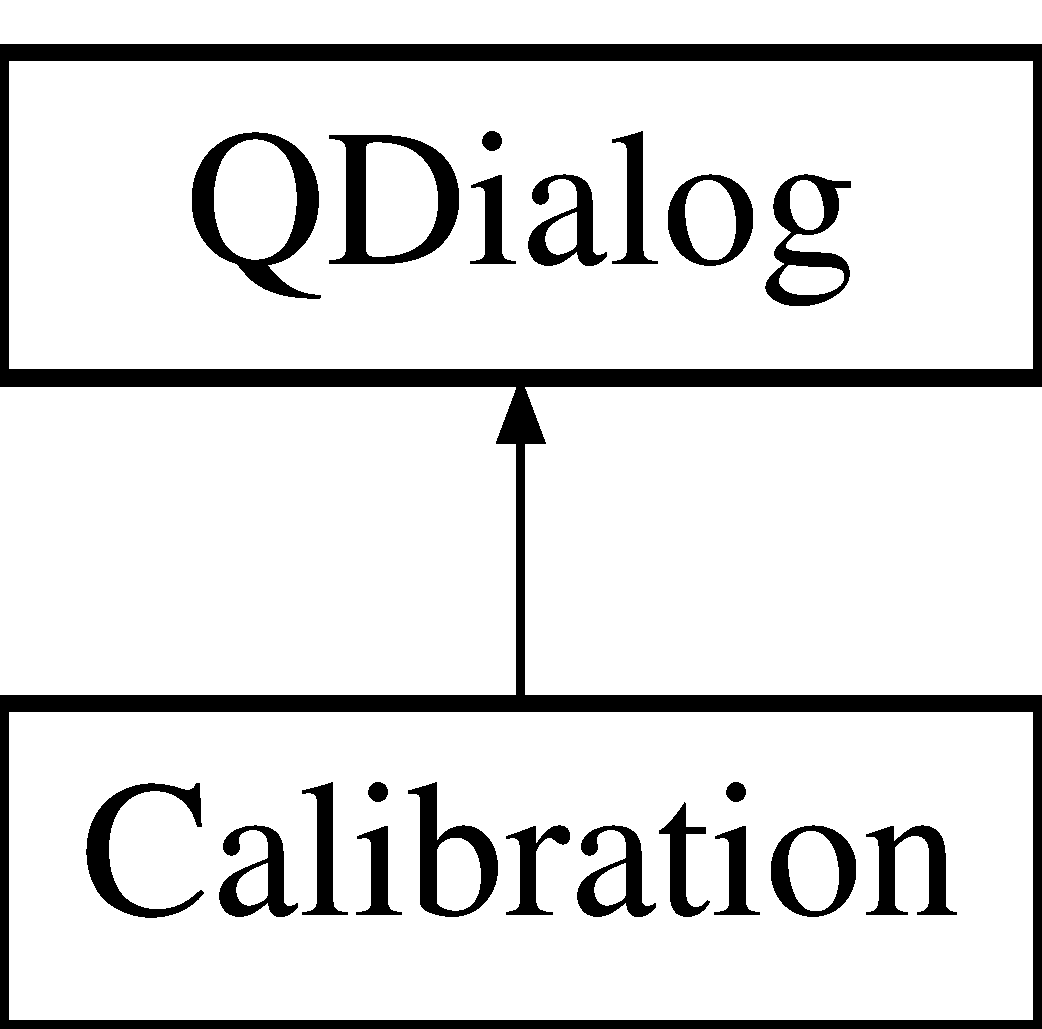
\includegraphics[height=2.000000cm]{classCalibration}
\end{center}
\end{figure}
\subsection*{Public Member Functions}
\begin{DoxyCompactItemize}
\item 
\hypertarget{classCalibration_a51dcbcaf05e8e841b0bcfb5511ba110c}{{\bfseries Calibration} (Q\-Widget $\ast$parent=0)}\label{classCalibration_a51dcbcaf05e8e841b0bcfb5511ba110c}

\item 
\hypertarget{classCalibration_a0c93ce32958eff964813d42ca517d730}{Ui\-::\-Calibration $\ast$ {\bfseries get\-Ui} ()}\label{classCalibration_a0c93ce32958eff964813d42ca517d730}

\item 
\hypertarget{classCalibration_a4d09685e8f5907b1be26edb8a5b0e060}{void {\bfseries show\-Data} ()}\label{classCalibration_a4d09685e8f5907b1be26edb8a5b0e060}

\item 
\hypertarget{classCalibration_ad5e1a103a408014eb62660e094443c54}{void {\bfseries save\-Plot} ()}\label{classCalibration_ad5e1a103a408014eb62660e094443c54}

\item 
\hypertarget{classCalibration_aeec90f8d9c81bf0ad91b35cc5db97331}{void {\bfseries get\-Calibration\-Parameters} ()}\label{classCalibration_aeec90f8d9c81bf0ad91b35cc5db97331}

\item 
\hypertarget{classCalibration_aa06e12a1921fa9b4f438a27a089d4436}{void {\bfseries show\-Table} ()}\label{classCalibration_aa06e12a1921fa9b4f438a27a089d4436}

\item 
\hypertarget{classCalibration_aecec6497e20fdd6236fefa3c39b53022}{void {\bfseries save\-Table\-Data} ()}\label{classCalibration_aecec6497e20fdd6236fefa3c39b53022}

\item 
\hypertarget{classCalibration_abfb479b712c0dc20a41f295d4353e8de}{virtual void {\bfseries accept} ()}\label{classCalibration_abfb479b712c0dc20a41f295d4353e8de}

\end{DoxyCompactItemize}


The documentation for this class was generated from the following file\-:\begin{DoxyCompactItemize}
\item 
/home/boris/\-Dropbox/dokumenty/\-S\-U\-R\-O/\-E\-U\-R\-A\-D\-O\-S\-\_\-school/intercomp/my\-\_\-program/qt\-\_\-application/alive/src/calibration.\-h\end{DoxyCompactItemize}

\hypertarget{classData}{\section{Data Class Reference}
\label{classData}\index{Data@{Data}}
}
\subsection*{Public Member Functions}
\begin{DoxyCompactItemize}
\item 
\hypertarget{classData_a1959550ffdd60408a174f2f9cd8ee2bd}{\hyperlink{classData}{Data} \& {\bfseries operator=} (const \hyperlink{classData}{Data} \&data)}\label{classData_a1959550ffdd60408a174f2f9cd8ee2bd}

\item 
\hypertarget{classData_a8a8a6c7d71ccb77a1ff4492db787996c}{string {\bfseries get\-Value} (const string a\-Var) const }\label{classData_a8a8a6c7d71ccb77a1ff4492db787996c}

\end{DoxyCompactItemize}
\subsection*{Static Public Member Functions}
\begin{DoxyCompactItemize}
\item 
\hypertarget{classData_abbc6642eda9d4960175ed812fb963fb3}{static const map$<$ string, \\*
string $>$ \& {\bfseries get\-Var\-Names\-Help} ()}\label{classData_abbc6642eda9d4960175ed812fb963fb3}

\end{DoxyCompactItemize}
\subsection*{Data Fields}
\begin{DoxyCompactItemize}
\item 
\hypertarget{classData_a3d3fcffaf58345b49b8ca51cfe71ac5c}{short {\bfseries Version}}\label{classData_a3d3fcffaf58345b49b8ca51cfe71ac5c}

\item 
\hypertarget{classData_ac834d7e12422de318f609e42286b4cda}{short {\bfseries Length}}\label{classData_ac834d7e12422de318f609e42286b4cda}

\item 
\hypertarget{classData_a7b8be3fa91c3ce1f0ea978291c8d44ed}{short {\bfseries Previous}}\label{classData_a7b8be3fa91c3ce1f0ea978291c8d44ed}

\item 
\hypertarget{classData_a549da9ef770d4de9090a63719a8205f7}{short {\bfseries N\-Points}}\label{classData_a549da9ef770d4de9090a63719a8205f7}

\item 
\hypertarget{classData_ad57f46e47c647eff3694d281d47d26c9}{int {\bfseries L\-Type}}\label{classData_ad57f46e47c647eff3694d281d47d26c9}

\item 
\hypertarget{classData_afd8f49a8c0c5b818af4b56b327b80ba1}{float {\bfseries Low}}\label{classData_afd8f49a8c0c5b818af4b56b327b80ba1}

\item 
\hypertarget{classData_abcfa6f65dfcf050bc3297c55c3263b4d}{float {\bfseries High}}\label{classData_abcfa6f65dfcf050bc3297c55c3263b4d}

\item 
\hypertarget{classData_a87604cbfa082e5480f6aba07db511c34}{float {\bfseries Rate}}\label{classData_a87604cbfa082e5480f6aba07db511c34}

\item 
\hypertarget{classData_a5e22baf811d8dd902f6cd74f0fda6fb3}{short {\bfseries Temperature}}\label{classData_a5e22baf811d8dd902f6cd74f0fda6fb3}

\item 
\hypertarget{classData_a442cbf09df631474b6c7332abd147986}{short {\bfseries X\-Coord}}\label{classData_a442cbf09df631474b6c7332abd147986}

\item 
\hypertarget{classData_aad59cf59fc2ba8c0f279230188f09f5b}{short {\bfseries Y\-Coord}}\label{classData_aad59cf59fc2ba8c0f279230188f09f5b}

\item 
\hypertarget{classData_a37d729a0baa295171625c510a003de47}{short {\bfseries Delay}}\label{classData_a37d729a0baa295171625c510a003de47}

\item 
\hypertarget{classData_a8c3b510401d81f718439d0c1311b90eb}{short {\bfseries On}}\label{classData_a8c3b510401d81f718439d0c1311b90eb}

\item 
\hypertarget{classData_a6c36df442580aee8cf5afba7a00f9b42}{short {\bfseries Off}}\label{classData_a6c36df442580aee8cf5afba7a00f9b42}

\item 
\hypertarget{classData_a211eeb9b20b42614ceb7d57b184cf8ca}{int {\bfseries Position}}\label{classData_a211eeb9b20b42614ceb7d57b184cf8ca}

\item 
\hypertarget{classData_abc812bd6aed8b378076078289e08064b}{int {\bfseries Run}}\label{classData_abc812bd6aed8b378076078289e08064b}

\item 
\hypertarget{classData_a6e91b1acd3ca6007cc5497f277dcb584}{char {\bfseries Time} \mbox{[}7\mbox{]}}\label{classData_a6e91b1acd3ca6007cc5497f277dcb584}

\item 
\hypertarget{classData_ad1b550d6ea4cfa2be1f1a8020bfbc47c}{char {\bfseries Date} \mbox{[}7\mbox{]}}\label{classData_ad1b550d6ea4cfa2be1f1a8020bfbc47c}

\item 
\hypertarget{classData_aa5b79093752274ef61d93e759b2f222d}{string {\bfseries Sequence}}\label{classData_aa5b79093752274ef61d93e759b2f222d}

\item 
\hypertarget{classData_ae9be542a2377f79c5da120f2c9041e28}{string {\bfseries User}}\label{classData_ae9be542a2377f79c5da120f2c9041e28}

\item 
\hypertarget{classData_a06a932d7f717dbf83fdf888528451249}{int {\bfseries Dtype}}\label{classData_a06a932d7f717dbf83fdf888528451249}

\item 
\hypertarget{classData_a1f3d0b34861e02310cd19576eee94f0d}{float {\bfseries I\-R\-R\-\_\-\-Time}}\label{classData_a1f3d0b34861e02310cd19576eee94f0d}

\item 
\hypertarget{classData_a12405989a9d14037e4dc3e7f89d7ba0d}{int {\bfseries I\-R\-R\-\_\-\-Type}}\label{classData_a12405989a9d14037e4dc3e7f89d7ba0d}

\item 
\hypertarget{classData_a9b3fa4cddd0e6bb375908f7e5107230c}{int {\bfseries I\-R\-R\-\_\-\-Unit}}\label{classData_a9b3fa4cddd0e6bb375908f7e5107230c}

\item 
\hypertarget{classData_a00fc7fa361fa6dedff7d76e1ebde40ba}{float {\bfseries Bl\-\_\-\-Time}}\label{classData_a00fc7fa361fa6dedff7d76e1ebde40ba}

\item 
\hypertarget{classData_aaf79ae3c53ea5888a4725e902887511c}{int {\bfseries Bl\-\_\-\-Unit}}\label{classData_aaf79ae3c53ea5888a4725e902887511c}

\item 
\hypertarget{classData_a354434fc3a6959cd0b83d3bc5bad0fc9}{float {\bfseries An\-\_\-\-Temp}}\label{classData_a354434fc3a6959cd0b83d3bc5bad0fc9}

\item 
\hypertarget{classData_a2368d01dc44c08133096e11594bdda34}{float {\bfseries An\-\_\-\-Time}}\label{classData_a2368d01dc44c08133096e11594bdda34}

\item 
\hypertarget{classData_a3f10a2c33dfabaa8e87c48a816fc686e}{int {\bfseries Norm1}}\label{classData_a3f10a2c33dfabaa8e87c48a816fc686e}

\item 
\hypertarget{classData_a9be797c58a600bb5bbb45aa452b9439d}{int {\bfseries Norm2}}\label{classData_a9be797c58a600bb5bbb45aa452b9439d}

\item 
\hypertarget{classData_ab4667f721032b27dcdbbd1eddf47c539}{int {\bfseries Norm3}}\label{classData_ab4667f721032b27dcdbbd1eddf47c539}

\item 
\hypertarget{classData_a9a9c8aae6f3b684cee95bb963c5efd39}{int {\bfseries B\-G}}\label{classData_a9a9c8aae6f3b684cee95bb963c5efd39}

\item 
\hypertarget{classData_ac9568462b2373d82c7cb61dd4c8917f1}{short {\bfseries Shift}}\label{classData_ac9568462b2373d82c7cb61dd4c8917f1}

\item 
\hypertarget{classData_a85eb6dc29671912d271abfbf87ba4668}{string {\bfseries Sample}}\label{classData_a85eb6dc29671912d271abfbf87ba4668}

\item 
\hypertarget{classData_a64e73b0e3724b524818866d40da36cdc}{string {\bfseries Comment}}\label{classData_a64e73b0e3724b524818866d40da36cdc}

\item 
\hypertarget{classData_ac62fd4b9f359c55f3b74986d17fb5466}{int {\bfseries Light\-Source}}\label{classData_ac62fd4b9f359c55f3b74986d17fb5466}

\item 
\hypertarget{classData_a33fe0e61968e172e8e6deeff18e312da}{int {\bfseries Set}}\label{classData_a33fe0e61968e172e8e6deeff18e312da}

\item 
\hypertarget{classData_a2ae38cd932d022cdaa6539270d796525}{int {\bfseries Tag}}\label{classData_a2ae38cd932d022cdaa6539270d796525}

\item 
\hypertarget{classData_ab96363bc246bbb3cf614bbbf833b25b9}{short {\bfseries Grain}}\label{classData_ab96363bc246bbb3cf614bbbf833b25b9}

\item 
\hypertarget{classData_aa13f8c639d99af74b1663c2a8bbb7290}{float {\bfseries Light\-Power}}\label{classData_aa13f8c639d99af74b1663c2a8bbb7290}

\item 
\hypertarget{classData_a29b16e359ec7f0beb0df4660a4babc52}{short {\bfseries System\-I\-D}}\label{classData_a29b16e359ec7f0beb0df4660a4babc52}

\item 
\hypertarget{classData_a6a6a1a08992c66c00b8689f6303d5dcb}{char {\bfseries R\-E\-S\-E\-R\-V\-E\-D\-\_\-3\-\_\-1} \mbox{[}36\mbox{]}}\label{classData_a6a6a1a08992c66c00b8689f6303d5dcb}

\item 
\hypertarget{classData_aa4e7c8485ef4be875a02f4e2d29ce31f}{float {\bfseries On\-Time}}\label{classData_aa4e7c8485ef4be875a02f4e2d29ce31f}

\item 
\hypertarget{classData_a726a901f27b51eadc77bc133f6cad31f}{float {\bfseries Off\-Time}}\label{classData_a726a901f27b51eadc77bc133f6cad31f}

\item 
\hypertarget{classData_ade5a9a45b64b00444756233294fa8578}{int {\bfseries Enable\-Flags}}\label{classData_ade5a9a45b64b00444756233294fa8578}

\item 
\hypertarget{classData_afd2a738f112e0d2ef1ccf73333b1f28c}{int {\bfseries On\-Gate\-Delay}}\label{classData_afd2a738f112e0d2ef1ccf73333b1f28c}

\item 
\hypertarget{classData_a5dd91559b54665da75f8bac7167620e1}{int {\bfseries Off\-Gate\-Delay}}\label{classData_a5dd91559b54665da75f8bac7167620e1}

\item 
\hypertarget{classData_a8623e1110c482a5d686e001102a4e8dc}{char {\bfseries R\-E\-S\-E\-R\-V\-E\-D\-\_\-3\-\_\-2}}\label{classData_a8623e1110c482a5d686e001102a4e8dc}

\item 
\hypertarget{classData_afa1c907a3bbd2cea47882d31aaf1a09a}{char {\bfseries R\-E\-S\-E\-R\-V\-E\-D\-\_\-4\-\_\-1} \mbox{[}20\mbox{]}}\label{classData_afa1c907a3bbd2cea47882d31aaf1a09a}

\item 
\hypertarget{classData_a3f0db92f4912583f0d97332433f382e4}{int {\bfseries Curve\-No}}\label{classData_a3f0db92f4912583f0d97332433f382e4}

\item 
\hypertarget{classData_a3913e79a18ae0e5ec0a2edd392d9cda0}{int {\bfseries Time\-Tick}}\label{classData_a3913e79a18ae0e5ec0a2edd392d9cda0}

\item 
\hypertarget{classData_ae9ee62ded9014c345cdcf747e04fe3f1}{int {\bfseries Stim\-Period}}\label{classData_ae9ee62ded9014c345cdcf747e04fe3f1}

\item 
\hypertarget{classData_aa318cff25bbd44f5167e1538482bd494}{int {\bfseries Gate\-Enabled}}\label{classData_aa318cff25bbd44f5167e1538482bd494}

\item 
\hypertarget{classData_aeab0c94e48521b9b6b5aa768638a3345}{int {\bfseries Gate\-Start}}\label{classData_aeab0c94e48521b9b6b5aa768638a3345}

\item 
\hypertarget{classData_a7f84b73053ee9d03380b3cb41e0684d2}{int {\bfseries Gate\-End}}\label{classData_a7f84b73053ee9d03380b3cb41e0684d2}

\item 
\hypertarget{classData_a6552ccf8b385e190bad656d0d655278f}{bool {\bfseries P\-Tenabled}}\label{classData_a6552ccf8b385e190bad656d0d655278f}

\item 
\hypertarget{classData_a73ef565807b045ff515c8342dc1fd3f5}{char {\bfseries R\-E\-S\-E\-R\-V\-E\-D\-\_\-4\-\_\-2} \mbox{[}10\mbox{]}}\label{classData_a73ef565807b045ff515c8342dc1fd3f5}

\item 
\hypertarget{classData_a55eca8496bfeb5d6d14d2f69a44c8eb1}{vector$<$ int $>$ {\bfseries D\-Points}}\label{classData_a55eca8496bfeb5d6d14d2f69a44c8eb1}

\item 
\hypertarget{classData_aa4febdde96d28f7740a30e0c2f58eff5}{int {\bfseries m\-Date\-Time}}\label{classData_aa4febdde96d28f7740a30e0c2f58eff5}

\item 
\hypertarget{classData_abf03ecd8788f1086e68bc33baf776c45}{int {\bfseries I\-R\-R\-\_\-\-Date\-Time}}\label{classData_abf03ecd8788f1086e68bc33baf776c45}

\item 
\hypertarget{classData_a96bec838c423f73e8c5a4ae71754d549}{struct tm {\bfseries Date\-Time}}\label{classData_a96bec838c423f73e8c5a4ae71754d549}

\item 
\hypertarget{classData_a8c2c5be33ab9680c7c3983e9e858b268}{double {\bfseries fad\-Parameters} \mbox{[}2\mbox{]}}\label{classData_a8c2c5be33ab9680c7c3983e9e858b268}

\item 
\hypertarget{classData_a6760cf2282a9a70bbf7e66e19479f4d9}{double {\bfseries e\-Fad\-Parameters} \mbox{[}2\mbox{]}}\label{classData_a6760cf2282a9a70bbf7e66e19479f4d9}

\item 
\hypertarget{classData_a6bcd68557e3ba799ade06fd96398b488}{double {\bfseries fad\-\_\-cov\-\_\-0\-\_\-1}}\label{classData_a6bcd68557e3ba799ade06fd96398b488}

\item 
\hypertarget{classData_a7fffccb3ce17db148bd32f868fec2aec}{gsl\-\_\-matrix $\ast$ {\bfseries fad\-Covariant\-Matrix}}\label{classData_a7fffccb3ce17db148bd32f868fec2aec}

\item 
\hypertarget{classData_abace911f0a2709d788bfce3be443c805}{Fad\-Function {\bfseries fad\-Function}}\label{classData_abace911f0a2709d788bfce3be443c805}

\item 
\hypertarget{classData_a0a2e114f10d5cba36a37c7bf15fa1ffb}{double {\bfseries range\-Signal} \mbox{[}2\mbox{]}}\label{classData_a0a2e114f10d5cba36a37c7bf15fa1ffb}

\item 
\hypertarget{classData_a9d770d30613f58eb573ac53524844538}{double {\bfseries range\-Background} \mbox{[}2\mbox{]}}\label{classData_a9d770d30613f58eb573ac53524844538}

\end{DoxyCompactItemize}
\subsection*{Static Public Attributes}
\begin{DoxyCompactItemize}
\item 
\hypertarget{classData_a6fc19df2521dfe5d739d6018b15326a3}{static const int {\bfseries T\-I\-M\-E\-D\-A\-T\-E\-\_\-\-S\-I\-Z\-E} =7}\label{classData_a6fc19df2521dfe5d739d6018b15326a3}

\item 
\hypertarget{classData_ac275d6a042ec7a06585702d43c8fbbca}{static const int {\bfseries U\-S\-E\-R\-\_\-\-S\-E\-Q\-U\-E\-N\-C\-E\-\_\-\-S\-I\-Z\-E} =9}\label{classData_ac275d6a042ec7a06585702d43c8fbbca}

\item 
\hypertarget{classData_a993296133daa1260f863fe67d9fac401}{static const int {\bfseries S\-A\-M\-P\-L\-E\-\_\-\-S\-I\-Z\-E} =21}\label{classData_a993296133daa1260f863fe67d9fac401}

\item 
\hypertarget{classData_a69d0299f85e7437d4f450122174a0259}{static const int {\bfseries C\-O\-M\-M\-E\-N\-T\-\_\-\-S\-I\-Z\-E} =81}\label{classData_a69d0299f85e7437d4f450122174a0259}

\item 
\hypertarget{classData_adb9405a86ea64e5a9b2ef2620db26ba7}{static const vector$<$ string $>$ {\bfseries L\-T\-Y\-P\-E}}\label{classData_adb9405a86ea64e5a9b2ef2620db26ba7}

\item 
\hypertarget{classData_ad74ba79472bc888594476cab4a7ace58}{static const vector$<$ string $>$ {\bfseries D\-T\-Y\-P\-E}}\label{classData_ad74ba79472bc888594476cab4a7ace58}

\item 
\hypertarget{classData_a51c7d7f85301f929304f813d92ce8669}{static const vector$<$ string $>$ {\bfseries L\-I\-G\-H\-T\-\_\-\-S\-O\-U\-R\-C\-E}}\label{classData_a51c7d7f85301f929304f813d92ce8669}

\item 
\hypertarget{classData_ac85a75fe45681718c87b323e9a898147}{static const vector$<$ string $>$ {\bfseries I\-R\-R\-\_\-\-T\-Y\-P\-E}}\label{classData_ac85a75fe45681718c87b323e9a898147}

\item 
\hypertarget{classData_a2139a4b080e0178ebe95cba97a185ac3}{static const vector$<$ string $>$ {\bfseries I\-R\-R\-\_\-\-U\-N\-I\-T}}\label{classData_a2139a4b080e0178ebe95cba97a185ac3}

\item 
\hypertarget{classData_a4d4ce75a1ee77aefa4b07fc1a1eb48de}{static const vector$<$ string $>$ {\bfseries B\-L\-\_\-\-U\-N\-I\-T}}\label{classData_a4d4ce75a1ee77aefa4b07fc1a1eb48de}

\item 
\hypertarget{classData_a7ab8ae598a0ca941084eeee32efaa020}{static const vector$<$ string $>$ {\bfseries F\-A\-D\-\_\-\-F\-O\-R\-M\-U\-L\-A}}\label{classData_a7ab8ae598a0ca941084eeee32efaa020}

\item 
\hypertarget{classData_a3f6d7e3759cb32957f672d89f05ab1c4}{static const vector$<$ string $>$ {\bfseries F\-A\-D\-\_\-\-F\-U\-N\-C\-T\-I\-O\-N\-S}}\label{classData_a3f6d7e3759cb32957f672d89f05ab1c4}

\item 
\hypertarget{classData_a61473370adeb3358cfe77f92f33435a7}{static const vector$<$ string $>$ {\bfseries V\-A\-R\-\_\-\-N\-A\-M\-E\-S}}\label{classData_a61473370adeb3358cfe77f92f33435a7}

\item 
\hypertarget{classData_a351402311bf9bc250c788e59b015841c}{static const vector$<$ string $>$ {\bfseries U\-S\-E\-R\-\_\-\-V\-A\-R\-\_\-\-N\-A\-M\-E\-S}}\label{classData_a351402311bf9bc250c788e59b015841c}

\end{DoxyCompactItemize}
\subsection*{Friends}
\begin{DoxyCompactItemize}
\item 
\hypertarget{classData_ac9e8b1958e329799e87880d3fab3df57}{ostream \& {\bfseries operator$<$$<$} (ostream \&stream, const \hyperlink{classData}{Data} \&a\-Data)}\label{classData_ac9e8b1958e329799e87880d3fab3df57}

\item 
\hypertarget{classData_a22dfb8fe66795dc99d59323402e68810}{ostream \& {\bfseries operator$<$$<$} (ostream \&stream, const \hyperlink{classData}{Data} $\ast$a\-Data)}\label{classData_a22dfb8fe66795dc99d59323402e68810}

\end{DoxyCompactItemize}


The documentation for this class was generated from the following file\-:\begin{DoxyCompactItemize}
\item 
/home/boris/\-Dropbox/dokumenty/\-S\-U\-R\-O/\-E\-U\-R\-A\-D\-O\-S\-\_\-school/intercomp/my\-\_\-program/qt\-\_\-application/alive/src/data.\-h\end{DoxyCompactItemize}

\hypertarget{classDataHandle}{\section{Data\-Handle Class Reference}
\label{classDataHandle}\index{Data\-Handle@{Data\-Handle}}
}
\subsection*{Public Member Functions}
\begin{DoxyCompactItemize}
\item 
\hypertarget{classDataHandle_ae1667fdd8c3e7dc4f949b828302fee0a}{const vector$<$ vector$<$ int $>$ $>$ \& {\bfseries get\-Data\-Points} ()}\label{classDataHandle_ae1667fdd8c3e7dc4f949b828302fee0a}

\item 
\hypertarget{classDataHandle_a0c73485b27cb84a81e8ce8687cadb0be}{const vector$<$ \hyperlink{classData}{Data} $>$ \& {\bfseries get\-Data} ()}\label{classDataHandle_a0c73485b27cb84a81e8ce8687cadb0be}

\item 
\hypertarget{classDataHandle_a6fa18d21b416a4a878734fdf80a51161}{int {\bfseries get\-Configuration\-Data} (const string \&conf\-Data\-Name)}\label{classDataHandle_a6fa18d21b416a4a878734fdf80a51161}

\item 
\hypertarget{classDataHandle_ae851018a34b27dd9864707078b3658a5}{const double $\ast$ {\bfseries get\-Fad\-Parameters} (const int which) const }\label{classDataHandle_ae851018a34b27dd9864707078b3658a5}

\item 
\hypertarget{classDataHandle_a39aa5ab26ae6cdad163aeede417ca7b8}{const double $\ast$ {\bfseries get\-E\-Fad\-Parameters} (const int which) const }\label{classDataHandle_a39aa5ab26ae6cdad163aeede417ca7b8}

\item 
\hypertarget{classDataHandle_a0409902e4f2fad832cca5f313db34ee0}{void {\bfseries set\-Fad\-Parameters} (const double $\ast$parameters, gsl\-\_\-matrix $\ast$fad\-Covariant\-Matrix, const Fad\-Function fad\-Function, const int which)}\label{classDataHandle_a0409902e4f2fad832cca5f313db34ee0}

\item 
\hypertarget{classDataHandle_ac6ff603576fc66ad42fa713109e046ae}{void {\bfseries set\-Data} (const vector$<$ \hyperlink{classData}{Data} $>$ data)}\label{classDataHandle_ac6ff603576fc66ad42fa713109e046ae}

\item 
\hypertarget{classDataHandle_a50550680c45eb39c456e189a622c284d}{void {\bfseries set\-Data\-Not\-Points} (const int which, const \hyperlink{classData}{Data} \&data)}\label{classDataHandle_a50550680c45eb39c456e189a622c284d}

\item 
\hypertarget{classDataHandle_a0e83770b88b152cb4e4f04658446e46d}{void {\bfseries set\-Range\-Signal\-Background} (const double $\ast$signal, const double $\ast$background, const int which)}\label{classDataHandle_a0e83770b88b152cb4e4f04658446e46d}

\item 
\hypertarget{classDataHandle_a1aee5afea4b6ad49fa6eeafa63696600}{set$<$ int $>$ {\bfseries get\-Which\-D\-Type} (const string \&which\-Type)}\label{classDataHandle_a1aee5afea4b6ad49fa6eeafa63696600}

\item 
\hypertarget{classDataHandle_a88984a5bf8769adecd11ec0df1dddce3}{\hyperlink{classBinReader}{Bin\-Reader} $\ast$ {\bfseries get\-Bin\-Reader} ()}\label{classDataHandle_a88984a5bf8769adecd11ec0df1dddce3}

\item 
\hypertarget{classDataHandle_a4ef0bd4b1ee9051b4a3d150b740dc6cd}{void {\bfseries create\-Data} (string name)}\label{classDataHandle_a4ef0bd4b1ee9051b4a3d150b740dc6cd}

\item 
\hypertarget{classDataHandle_a03cfb29618f9d46d4c1207ecfb9a743f}{void {\bfseries create\-Db} (const Q\-String db\-Name, const Q\-String user\-Name=\char`\"{}root\char`\"{}, const Q\-String host\-Name=\char`\"{}localhost\char`\"{}, const Q\-String password=\char`\"{}\char`\"{})}\label{classDataHandle_a03cfb29618f9d46d4c1207ecfb9a743f}

\item 
\hypertarget{classDataHandle_a5510a603caa75344006b1d8d74e801df}{pair$<$ double, double $>$ {\bfseries compute\-General\-Dose} (const pair$<$ double, double $>$ \&signal, Function function, const double resolution=1e-\/1)}\label{classDataHandle_a5510a603caa75344006b1d8d74e801df}

\item 
\hypertarget{classDataHandle_a9ee8fcf0076b08f37c6276cdc47a8973}{pair$<$ double, double $>$ {\bfseries compute\-Fad\-Corr} (const int which, const Fad\-Function fad\-Func) const }\label{classDataHandle_a9ee8fcf0076b08f37c6276cdc47a8973}

\item 
\hypertarget{classDataHandle_ae8f3562cfc85d429977c4fb6dc5559a1}{double {\bfseries get\-Integral} (const int which, const double $\ast$integral\-Range) const }\label{classDataHandle_ae8f3562cfc85d429977c4fb6dc5559a1}

\item 
\hypertarget{classDataHandle_a923935abbf57334773e277fe78960c19}{std\-::pair$<$ double, double $>$ {\bfseries get\-Signal} (const int which, const double $\ast$signal\-Range=N\-U\-L\-L, const double $\ast$background\-Range=N\-U\-L\-L)}\label{classDataHandle_a923935abbf57334773e277fe78960c19}

\item 
\hypertarget{classDataHandle_a969c18ae3f2bc8782ab02959a244e965}{void {\bfseries set\-Main\-Window\-Data} (\hyperlink{structMainWindowData}{Main\-Window\-Data} \&data)}\label{classDataHandle_a969c18ae3f2bc8782ab02959a244e965}

\item 
\hypertarget{classDataHandle_af005735776acdb074212d5c82224a306}{const double $\ast$ {\bfseries compute\-Calibration} (const double $\ast$signal\-Range=N\-U\-L\-L, const double $\ast$background\-Range=N\-U\-L\-L, Function function=Linear)}\label{classDataHandle_af005735776acdb074212d5c82224a306}

\item 
\hypertarget{classDataHandle_a8aebf9e31648489bed13d51ca965a91a}{const double $\ast$ {\bfseries chi\-Square\-Compute\-G\-S\-L} (const vector$<$ pair$<$ pair$<$ double, double $>$, pair$<$ double, double $>$ $>$ $>$ \&input\-Data, Function function)}\label{classDataHandle_a8aebf9e31648489bed13d51ca965a91a}

\item 
\hypertarget{classDataHandle_aeeedcdce39700e848e80bef4f3d70a69}{const double $\ast$ {\bfseries get\-Parameters} () const }\label{classDataHandle_aeeedcdce39700e848e80bef4f3d70a69}

\item 
\hypertarget{classDataHandle_ab020432837359dc871d483c329aa6f2b}{const gsl\-\_\-matrix $\ast$ {\bfseries get\-Covariant\-Matrix} () const }\label{classDataHandle_ab020432837359dc871d483c329aa6f2b}

\item 
\hypertarget{classDataHandle_ad27a12a6bd6bb3b72c4ea008599c7de1}{Q\-Sql\-Database \& {\bfseries get\-Db} ()}\label{classDataHandle_ad27a12a6bd6bb3b72c4ea008599c7de1}

\item 
\hypertarget{classDataHandle_a138330c0f643216df97c21ba9a66f39d}{const \hyperlink{structMainWindowData}{Main\-Window\-Data} \& {\bfseries get\-Main\-Window\-Data} ()}\label{classDataHandle_a138330c0f643216df97c21ba9a66f39d}

\item 
\hypertarget{classDataHandle_a43f94cde8228583790f7c279df9ef8e8}{double {\bfseries get\-Dose\-Unc} (const double signal, const double $\ast$calibration\-Parameters) const }\label{classDataHandle_a43f94cde8228583790f7c279df9ef8e8}

\item 
\hypertarget{classDataHandle_a2273fbb63ac6b5b88f2fcd10b6578a24}{const double $\ast$ {\bfseries get\-Initial\-Parameters} () const }\label{classDataHandle_a2273fbb63ac6b5b88f2fcd10b6578a24}

\item 
\hypertarget{classDataHandle_a6ded2edbe17f9dc2ceeb6306c0ae4684}{void {\bfseries set\-Initial\-Parameters} (const double $\ast$initial\-Parameters)}\label{classDataHandle_a6ded2edbe17f9dc2ceeb6306c0ae4684}

\item 
\hypertarget{classDataHandle_a5f8951671ff5d22b39c0e85931552135}{const vector$<$ vector$<$ int $>$ $>$ \& {\bfseries get\-Values} () const }\label{classDataHandle_a5f8951671ff5d22b39c0e85931552135}

\item 
\hypertarget{classDataHandle_a6eda37bc92ad512e273d341aff1abbd7}{void {\bfseries set\-Values} (vector$<$ vector$<$ int $>$ $>$ \&values)}\label{classDataHandle_a6eda37bc92ad512e273d341aff1abbd7}

\item 
\hypertarget{classDataHandle_a16aa7bd6d05c938a919e8c36a570890d}{void {\bfseries set\-Used\-Measurements} (const set$<$ int $>$ measurements)}\label{classDataHandle_a16aa7bd6d05c938a919e8c36a570890d}

\item 
\hypertarget{classDataHandle_a8dd3496a7e7c942f5833f074a4045d3b}{const set$<$ int $>$ \& {\bfseries get\-Used\-Measurements} ()}\label{classDataHandle_a8dd3496a7e7c942f5833f074a4045d3b}

\item 
\hypertarget{classDataHandle_a34932be9a3d0e4dd5eaf1ebc6644c65d}{void {\bfseries set\-Fad\-Correction} (const pair$<$ double, double $>$ \&fad\-Correction)}\label{classDataHandle_a34932be9a3d0e4dd5eaf1ebc6644c65d}

\item 
\hypertarget{classDataHandle_ae42ee5520c137810b47aae715a61b5e4}{const pair$<$ double, double $>$ \& {\bfseries get\-Fad\-Correction} () const }\label{classDataHandle_ae42ee5520c137810b47aae715a61b5e4}

\item 
\hypertarget{classDataHandle_a9ce1a40b516cbdce59cafee6d51e9cde}{void {\bfseries set\-Time\-Unit} (const Time\-Unit time\-Unit)}\label{classDataHandle_a9ce1a40b516cbdce59cafee6d51e9cde}

\item 
\hypertarget{classDataHandle_a0337fa2debd248143d1768223e39c34d}{Time\-Unit {\bfseries get\-Time\-Unit} () const }\label{classDataHandle_a0337fa2debd248143d1768223e39c34d}

\item 
\hypertarget{classDataHandle_a1955ab18952eddd0523e11d0bb786323}{void {\bfseries set\-Function} (const Function function)}\label{classDataHandle_a1955ab18952eddd0523e11d0bb786323}

\item 
\hypertarget{classDataHandle_aa42c616fdecac50471e58244caa24bbd}{Function {\bfseries get\-Function} () const }\label{classDataHandle_aa42c616fdecac50471e58244caa24bbd}

\item 
\hypertarget{classDataHandle_a845b2bb0537fb34e4ad037beb453e36b}{void {\bfseries set\-Database\-Path} (const string \&database\-Path)}\label{classDataHandle_a845b2bb0537fb34e4ad037beb453e36b}

\item 
\hypertarget{classDataHandle_a0a6efa3f5bc4f09a72299135e91b7c36}{const string \& {\bfseries get\-Database\-Path} () const }\label{classDataHandle_a0a6efa3f5bc4f09a72299135e91b7c36}

\item 
\hypertarget{classDataHandle_a302e1fc204cb37b5bb5ad339e8366160}{void {\bfseries set\-Database\-Name} (const string \&database\-Name)}\label{classDataHandle_a302e1fc204cb37b5bb5ad339e8366160}

\item 
\hypertarget{classDataHandle_aea4035af37d6f02460fcabd3667738f9}{const string \& {\bfseries get\-Database\-Name} () const }\label{classDataHandle_aea4035af37d6f02460fcabd3667738f9}

\item 
\hypertarget{classDataHandle_a3c279ceb4671d757033fa1211f594bff}{pair$<$ double, double $>$ {\bfseries get\-Dose\-Corrected} (const pair$<$ double, double $>$ \&dose\-Unc, const pair$<$ double, double $>$ fad\-Correction=pair$<$ double, double $>$(0, 0))}\label{classDataHandle_a3c279ceb4671d757033fa1211f594bff}

\end{DoxyCompactItemize}
\subsection*{Static Public Member Functions}
\begin{DoxyCompactItemize}
\item 
\hypertarget{classDataHandle_ace9a04d469e246e810d0953801eed10c}{static \hyperlink{classDataHandle}{Data\-Handle} $\ast$ {\bfseries get\-Instance} ()}\label{classDataHandle_ace9a04d469e246e810d0953801eed10c}

\item 
\hypertarget{classDataHandle_af126956f60c91b8a1a6e05c5d43c1c99}{static T\-O\-O\-L\-S\-::func {\bfseries get\-Function} (Function function)}\label{classDataHandle_af126956f60c91b8a1a6e05c5d43c1c99}

\item 
\hypertarget{classDataHandle_af87301e4edc221aefa777be9ec348368}{static T\-O\-O\-L\-S\-::fad\-Func {\bfseries get\-Fad\-Function} (Fad\-Function function)}\label{classDataHandle_af87301e4edc221aefa777be9ec348368}

\item 
\hypertarget{classDataHandle_ab0c8ed010b5f8a04bbb6bfa0055cda3b}{static T\-O\-O\-L\-S\-::e\-Fad\-Func {\bfseries get\-E\-Fad\-Function} (E\-Fad\-Function function)}\label{classDataHandle_ab0c8ed010b5f8a04bbb6bfa0055cda3b}

\end{DoxyCompactItemize}
\subsection*{Static Public Attributes}
\begin{DoxyCompactItemize}
\item 
\hypertarget{classDataHandle_a7cefcf02c9a59b111225dfc5491a8160}{static const vector$<$ string $>$ {\bfseries F\-I\-T\-\_\-\-F\-U\-N\-C\-T\-I\-O\-N\-S}}\label{classDataHandle_a7cefcf02c9a59b111225dfc5491a8160}

\item 
\hypertarget{classDataHandle_a8ea25e4b96194720f7f1133d9b560637}{static const vector$<$ string $>$ {\bfseries F\-I\-T\-\_\-\-F\-O\-R\-M\-U\-L\-A}}\label{classDataHandle_a8ea25e4b96194720f7f1133d9b560637}

\item 
\hypertarget{classDataHandle_af754b84ee488b481af4f4ada4e7c7a97}{static bool {\bfseries I\-S\-\_\-\-N\-E\-W}}\label{classDataHandle_af754b84ee488b481af4f4ada4e7c7a97}

\end{DoxyCompactItemize}
\subsection*{Friends}
\begin{DoxyCompactItemize}
\item 
\hypertarget{classDataHandle_a1e7c71a630f82999e0d0899a03a17f2b}{ostream \& {\bfseries operator$<$$<$} (ostream \&stream, const \hyperlink{classDataHandle}{Data\-Handle} \&data\-Handle)}\label{classDataHandle_a1e7c71a630f82999e0d0899a03a17f2b}

\item 
\hypertarget{classDataHandle_a405632c8edc40837fe270361ea4a7d05}{ostream \& {\bfseries operator$<$$<$} (ostream \&stream, const \hyperlink{classDataHandle}{Data\-Handle} $\ast$data\-Handle)}\label{classDataHandle_a405632c8edc40837fe270361ea4a7d05}

\end{DoxyCompactItemize}


The documentation for this class was generated from the following file\-:\begin{DoxyCompactItemize}
\item 
/home/boris/\-Dropbox/dokumenty/\-S\-U\-R\-O/\-E\-U\-R\-A\-D\-O\-S\-\_\-school/intercomp/my\-\_\-program/qt\-\_\-application/alive/src/datahandle.\-h\end{DoxyCompactItemize}

\hypertarget{classDbSave}{\section{Db\-Save Class Reference}
\label{classDbSave}\index{Db\-Save@{Db\-Save}}
}
Inheritance diagram for Db\-Save\-:\begin{figure}[H]
\begin{center}
\leavevmode
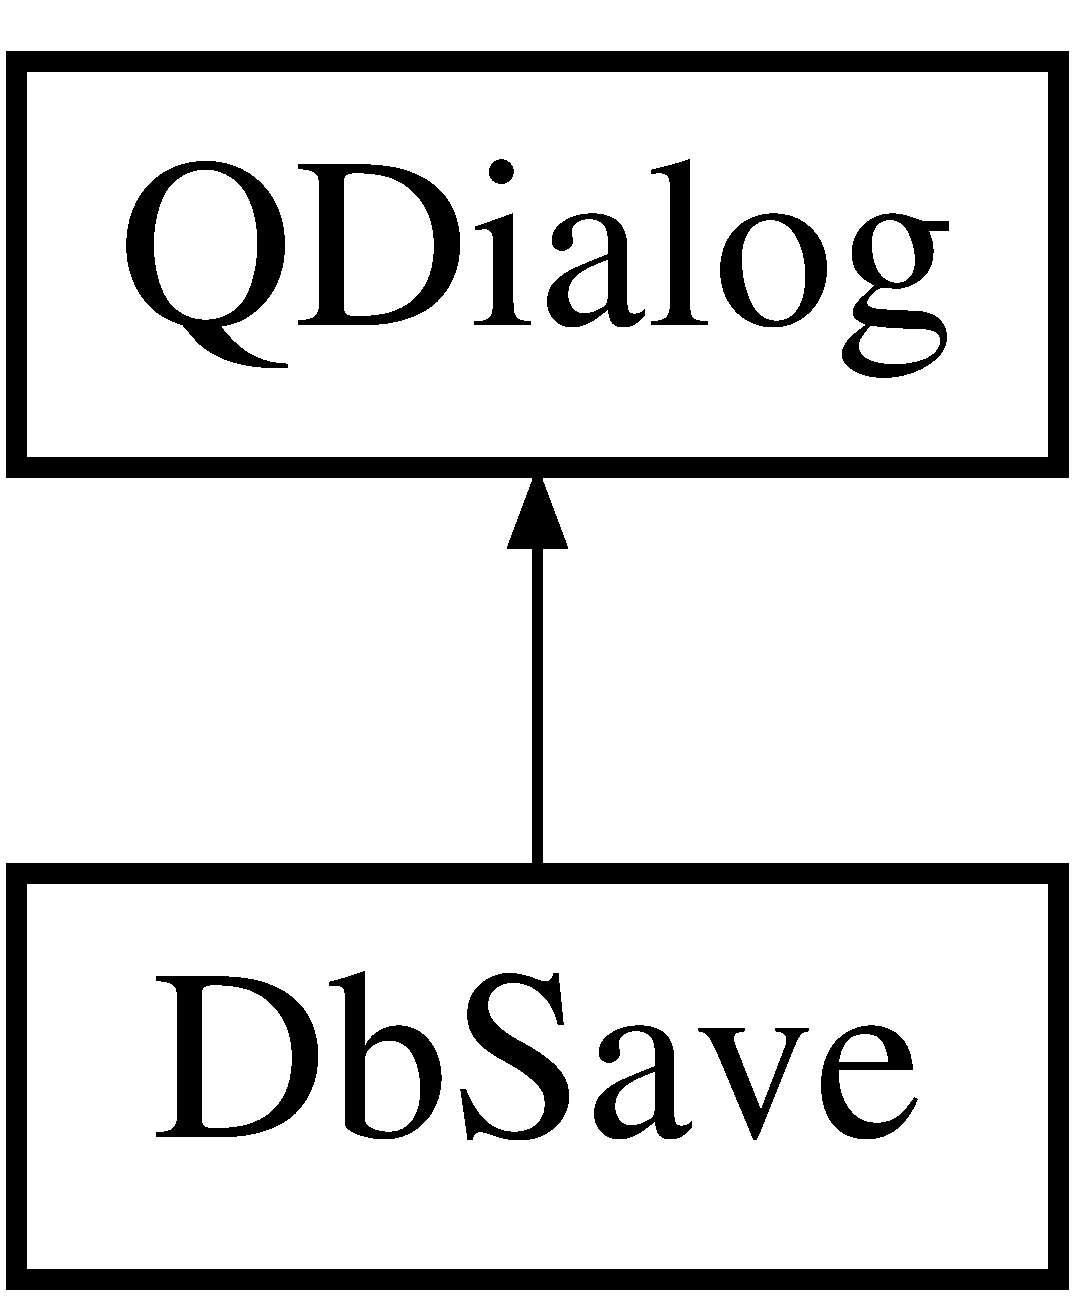
\includegraphics[height=2.000000cm]{classDbSave}
\end{center}
\end{figure}
\subsection*{Public Member Functions}
\begin{DoxyCompactItemize}
\item 
\hypertarget{classDbSave_a1cfb1f1272dd81fc3dd9451701471c98}{{\bfseries Db\-Save} (Q\-Widget $\ast$parent=0, int I\-D=0)}\label{classDbSave_a1cfb1f1272dd81fc3dd9451701471c98}

\end{DoxyCompactItemize}
\subsection*{Data Fields}
\begin{DoxyCompactItemize}
\item 
\hypertarget{classDbSave_a249538c80ad9ad31a9daf0d7ff99b646}{\hyperlink{classMyThread}{My\-Thread} $\ast$ {\bfseries \-\_\-my\-Thread}}\label{classDbSave_a249538c80ad9ad31a9daf0d7ff99b646}

\end{DoxyCompactItemize}


The documentation for this class was generated from the following file\-:\begin{DoxyCompactItemize}
\item 
/home/boris/\-Dropbox/dokumenty/\-S\-U\-R\-O/\-E\-U\-R\-A\-D\-O\-S\-\_\-school/intercomp/my\-\_\-program/qt\-\_\-application/alive/src/dbsave.\-h\end{DoxyCompactItemize}

\hypertarget{classInfo}{\section{Info Class Reference}
\label{classInfo}\index{Info@{Info}}
}
Inheritance diagram for Info\-:\begin{figure}[H]
\begin{center}
\leavevmode
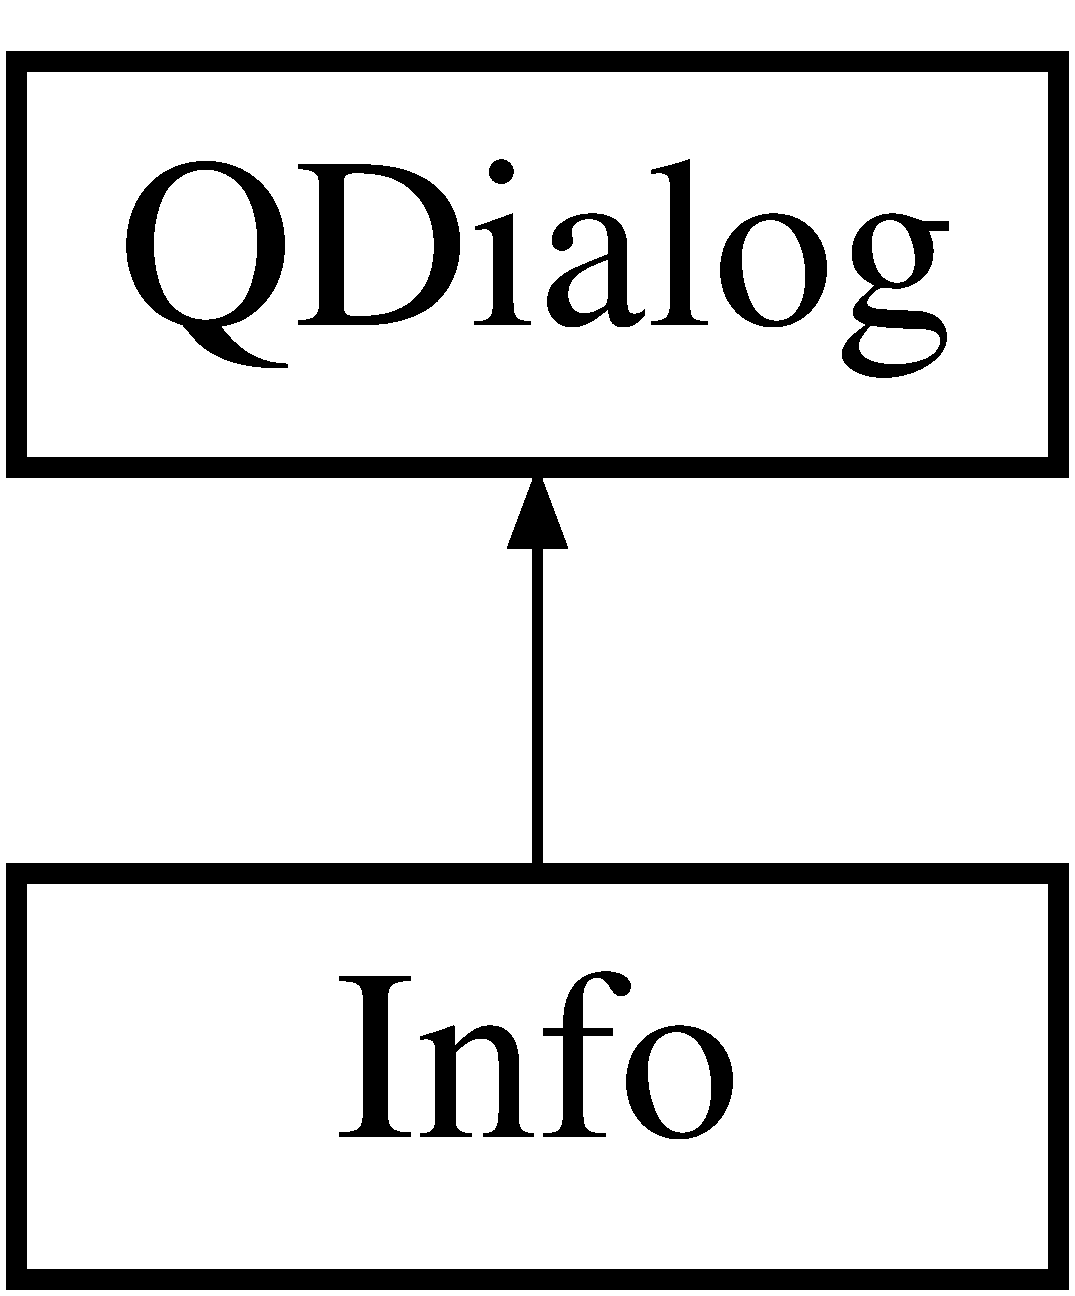
\includegraphics[height=2.000000cm]{classInfo}
\end{center}
\end{figure}
\subsection*{Public Slots}
\begin{DoxyCompactItemize}
\item 
\hypertarget{classInfo_af2626d1846ef58d75ff58a5dbade84ef}{virtual void {\bfseries accept} ()}\label{classInfo_af2626d1846ef58d75ff58a5dbade84ef}

\end{DoxyCompactItemize}
\subsection*{Public Member Functions}
\begin{DoxyCompactItemize}
\item 
\hypertarget{classInfo_abea2d82fa21531ecea0122a107ef183a}{{\bfseries Info} (Q\-Widget $\ast$parent=0)}\label{classInfo_abea2d82fa21531ecea0122a107ef183a}

\item 
\hypertarget{classInfo_a8c9adb529faf385cbcf753b38b5fa6fd}{void {\bfseries set\-U\-I\-Data} (int which)}\label{classInfo_a8c9adb529faf385cbcf753b38b5fa6fd}

\item 
\hypertarget{classInfo_a4198e1508cd99f933ff22ebee8578b82}{void {\bfseries store\-Data} ()}\label{classInfo_a4198e1508cd99f933ff22ebee8578b82}

\end{DoxyCompactItemize}


The documentation for this class was generated from the following file\-:\begin{DoxyCompactItemize}
\item 
/home/boris/\-Dropbox/dokumenty/\-S\-U\-R\-O/\-E\-U\-R\-A\-D\-O\-S\-\_\-school/intercomp/my\-\_\-program/qt\-\_\-application/alive/src/info.\-h\end{DoxyCompactItemize}

\hypertarget{classMainWindow}{\section{Main\-Window Class Reference}
\label{classMainWindow}\index{Main\-Window@{Main\-Window}}
}
Inheritance diagram for Main\-Window\-:\begin{figure}[H]
\begin{center}
\leavevmode
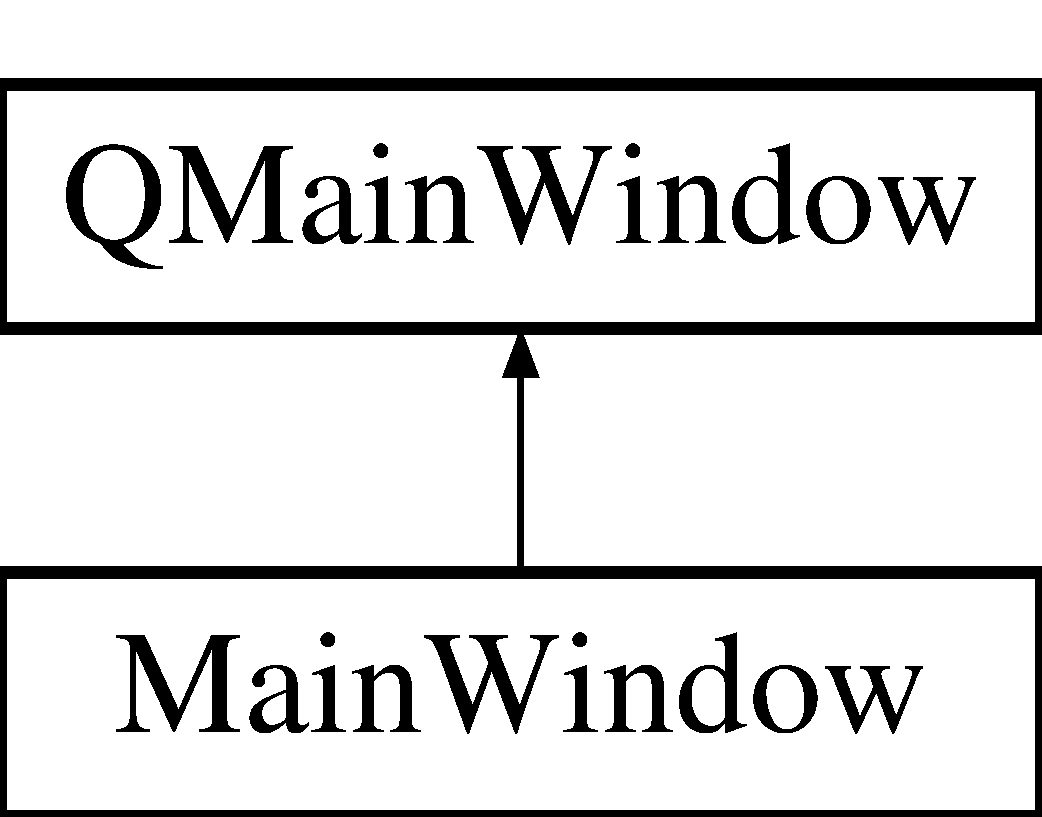
\includegraphics[height=2.000000cm]{classMainWindow}
\end{center}
\end{figure}
\subsection*{Signals}
\begin{DoxyCompactItemize}
\item 
\hypertarget{classMainWindow_a9bae38f96fcaedf7125b6264f289997a}{void {\bfseries saved\-Db\-Measurement} (int I\-D)}\label{classMainWindow_a9bae38f96fcaedf7125b6264f289997a}

\end{DoxyCompactItemize}
\subsection*{Public Member Functions}
\begin{DoxyCompactItemize}
\item 
\hypertarget{classMainWindow_a8b244be8b7b7db1b08de2a2acb9409db}{{\bfseries Main\-Window} (Q\-Widget $\ast$parent=0)}\label{classMainWindow_a8b244be8b7b7db1b08de2a2acb9409db}

\item 
\hypertarget{classMainWindow_a0392dad1c5a2be0720a06c1d7a5f5323}{void {\bfseries show\-U\-I\-Data} ()}\label{classMainWindow_a0392dad1c5a2be0720a06c1d7a5f5323}

\item 
\hypertarget{classMainWindow_afc1a58cf1884228025fc356943333c1b}{void {\bfseries show\-Table} ()}\label{classMainWindow_afc1a58cf1884228025fc356943333c1b}

\item 
\hypertarget{classMainWindow_a174a97382f475227fdf27c22b407e890}{void {\bfseries show\-Plot} ()}\label{classMainWindow_a174a97382f475227fdf27c22b407e890}

\item 
\hypertarget{classMainWindow_a15b3fb06da036220ff52460053ef5f9f}{void {\bfseries save\-Plot} ()}\label{classMainWindow_a15b3fb06da036220ff52460053ef5f9f}

\end{DoxyCompactItemize}
\subsection*{Static Public Attributes}
\begin{DoxyCompactItemize}
\item 
\hypertarget{classMainWindow_aa26df84f6e0c27464332427cec49d8a9}{static Q\-String {\bfseries T\-I\-T\-L\-E}}\label{classMainWindow_aa26df84f6e0c27464332427cec49d8a9}

\end{DoxyCompactItemize}


The documentation for this class was generated from the following file\-:\begin{DoxyCompactItemize}
\item 
/home/boris/\-Dropbox/dokumenty/\-S\-U\-R\-O/\-E\-U\-R\-A\-D\-O\-S\-\_\-school/intercomp/my\-\_\-program/qt\-\_\-application/alive/src/mainwindow.\-h\end{DoxyCompactItemize}

\hypertarget{structMainWindowData}{\section{Main\-Window\-Data Struct Reference}
\label{structMainWindowData}\index{Main\-Window\-Data@{Main\-Window\-Data}}
}
\subsection*{Data Fields}
\begin{DoxyCompactItemize}
\item 
\hypertarget{structMainWindowData_a13e994aac6efee77384aadf76389582c}{string {\bfseries name}}\label{structMainWindowData_a13e994aac6efee77384aadf76389582c}

\item 
\hypertarget{structMainWindowData_a3a1ed9bff4936fc9560c58c9d7cee92b}{string {\bfseries db\-Name}}\label{structMainWindowData_a3a1ed9bff4936fc9560c58c9d7cee92b}

\item 
\hypertarget{structMainWindowData_ae7731484e12a6e36e2d8e5415a0cad31}{string {\bfseries user}}\label{structMainWindowData_ae7731484e12a6e36e2d8e5415a0cad31}

\item 
\hypertarget{structMainWindowData_a84348f79f55b9c9da3b9c2d892f86a51}{double {\bfseries I\-R\-R\-\_\-\-Power}}\label{structMainWindowData_a84348f79f55b9c9da3b9c2d892f86a51}

\end{DoxyCompactItemize}


The documentation for this struct was generated from the following file\-:\begin{DoxyCompactItemize}
\item 
/home/boris/\-Dropbox/dokumenty/\-S\-U\-R\-O/\-E\-U\-R\-A\-D\-O\-S\-\_\-school/intercomp/my\-\_\-program/qt\-\_\-application/alive/src/datahandle.\-h\end{DoxyCompactItemize}

\hypertarget{classMyThread}{\section{My\-Thread Class Reference}
\label{classMyThread}\index{My\-Thread@{My\-Thread}}
}
Inheritance diagram for My\-Thread\-:\begin{figure}[H]
\begin{center}
\leavevmode
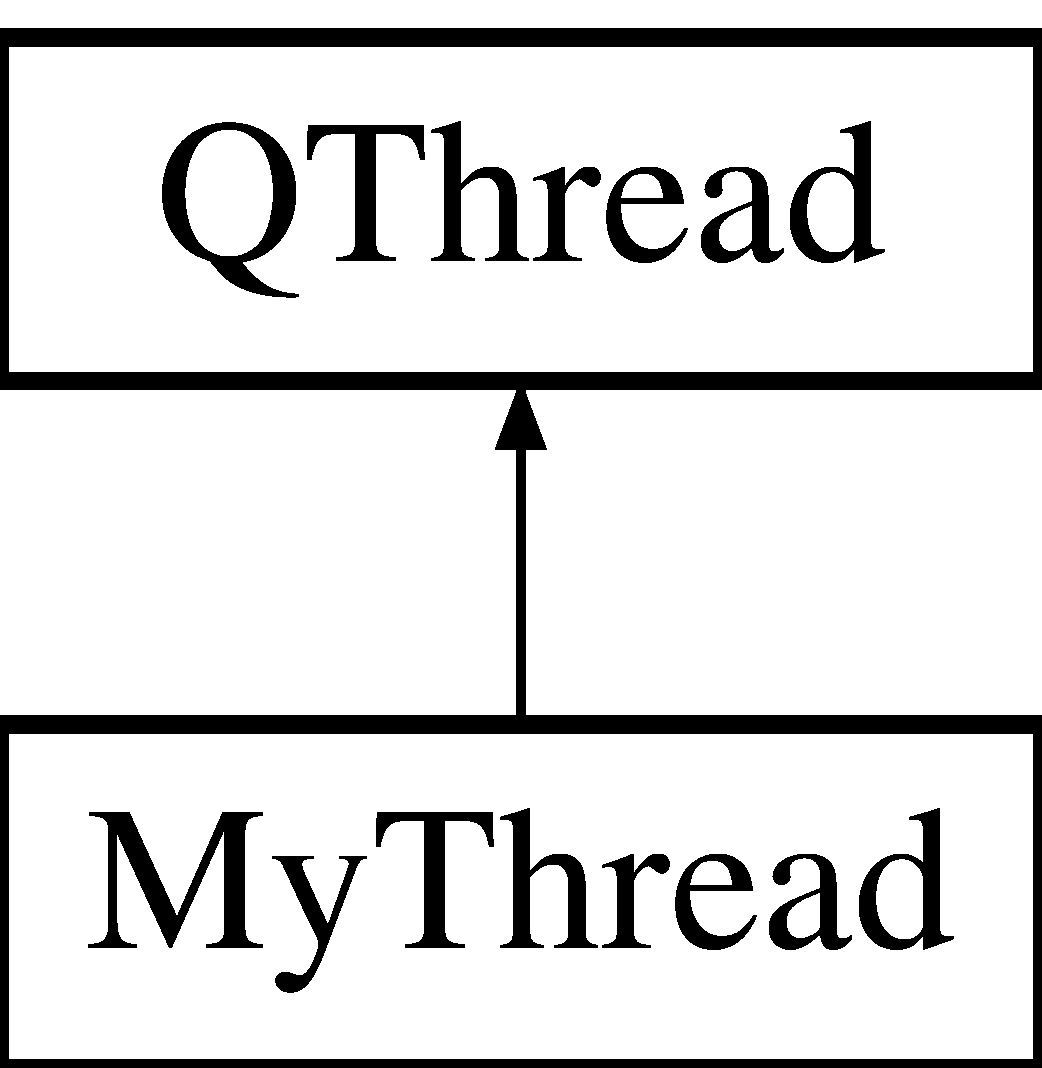
\includegraphics[height=2.000000cm]{classMyThread}
\end{center}
\end{figure}
\subsection*{Signals}
\begin{DoxyCompactItemize}
\item 
\hypertarget{classMyThread_ababaa32d071ee6f4c7e48a33ca31b103}{void {\bfseries db\-Saved} (int)}\label{classMyThread_ababaa32d071ee6f4c7e48a33ca31b103}

\end{DoxyCompactItemize}
\subsection*{Public Member Functions}
\begin{DoxyCompactItemize}
\item 
\hypertarget{classMyThread_ae06b3668f170ba0a0d61036d493ada39}{{\bfseries My\-Thread} (const int id, Q\-Object $\ast$parent=0)}\label{classMyThread_ae06b3668f170ba0a0d61036d493ada39}

\item 
\hypertarget{classMyThread_a9489f5226b5eda4dd811b05c0060613a}{virtual void {\bfseries run} ()}\label{classMyThread_a9489f5226b5eda4dd811b05c0060613a}

\end{DoxyCompactItemize}


The documentation for this class was generated from the following file\-:\begin{DoxyCompactItemize}
\item 
/home/boris/\-Dropbox/dokumenty/\-S\-U\-R\-O/\-E\-U\-R\-A\-D\-O\-S\-\_\-school/intercomp/my\-\_\-program/qt\-\_\-application/alive/src/mythread.\-h\end{DoxyCompactItemize}

\hypertarget{classPlateau}{\section{Plateau Class Reference}
\label{classPlateau}\index{Plateau@{Plateau}}
}
Inheritance diagram for Plateau\-:\begin{figure}[H]
\begin{center}
\leavevmode
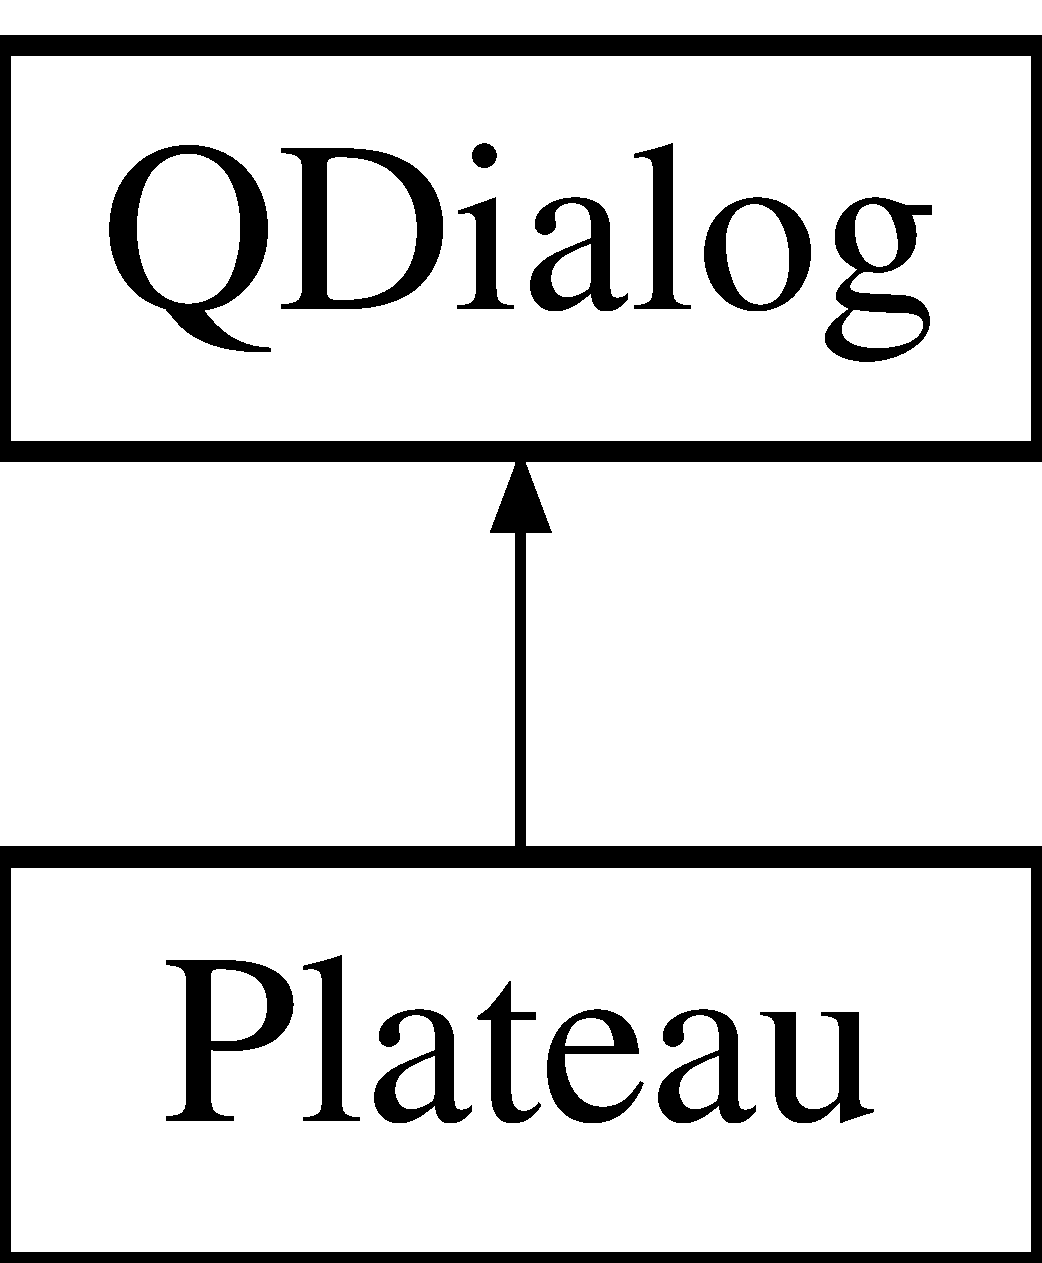
\includegraphics[height=2.000000cm]{classPlateau}
\end{center}
\end{figure}
\subsection*{Public Member Functions}
\begin{DoxyCompactItemize}
\item 
\hypertarget{classPlateau_a6da1eaad5e515d26fb11844fd8960c28}{{\bfseries Plateau} (Q\-Widget $\ast$parent=0)}\label{classPlateau_a6da1eaad5e515d26fb11844fd8960c28}

\item 
\hypertarget{classPlateau_afbf5a339d15b7916989617e04504986d}{const Ui\-::\-Plateau $\ast$ {\bfseries get\-Ui} ()}\label{classPlateau_afbf5a339d15b7916989617e04504986d}

\item 
\hypertarget{classPlateau_a8dd026299ed1c5ee5d516129baeb8bf2}{void {\bfseries save\-Plateau\-Plot} ()}\label{classPlateau_a8dd026299ed1c5ee5d516129baeb8bf2}

\end{DoxyCompactItemize}


The documentation for this class was generated from the following file\-:\begin{DoxyCompactItemize}
\item 
/home/boris/\-Dropbox/dokumenty/\-S\-U\-R\-O/\-E\-U\-R\-A\-D\-O\-S\-\_\-school/intercomp/my\-\_\-program/qt\-\_\-application/alive/src/plateau.\-h\end{DoxyCompactItemize}

\hypertarget{classSqlConnection}{\section{Sql\-Connection Class Reference}
\label{classSqlConnection}\index{Sql\-Connection@{Sql\-Connection}}
}
Inheritance diagram for Sql\-Connection\-:\begin{figure}[H]
\begin{center}
\leavevmode
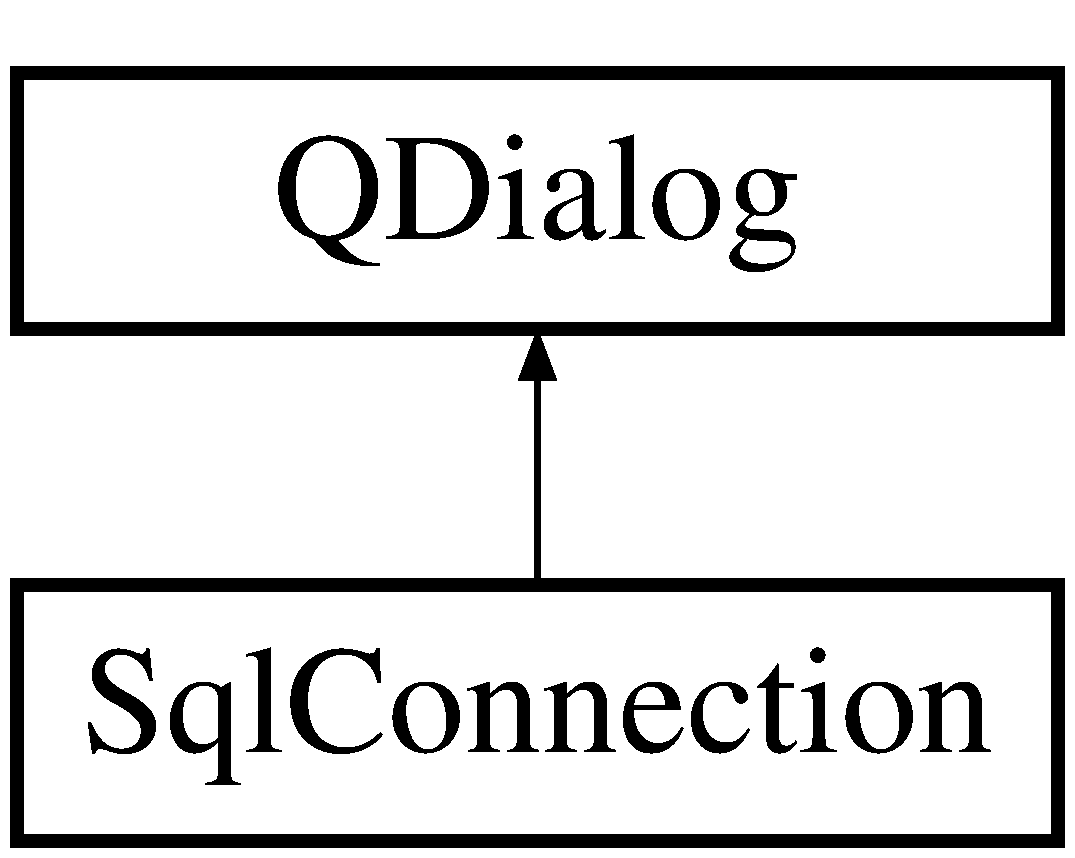
\includegraphics[height=2.000000cm]{classSqlConnection}
\end{center}
\end{figure}
\subsection*{Public Slots}
\begin{DoxyCompactItemize}
\item 
\hypertarget{classSqlConnection_a82e3b42ecea79904550546acbcef70b7}{void {\bfseries update\-Table\-From\-Command} ()}\label{classSqlConnection_a82e3b42ecea79904550546acbcef70b7}

\item 
\hypertarget{classSqlConnection_ade9e50f4c19e51e1229c2c71f0ae7be4}{void {\bfseries show\-Table} (const Q\-String \&t)}\label{classSqlConnection_ade9e50f4c19e51e1229c2c71f0ae7be4}

\item 
\hypertarget{classSqlConnection_a42fec1968d2a28aed8a130a3851715ee}{void {\bfseries on\-\_\-action\-Fetch\-Db\-\_\-triggered} ()}\label{classSqlConnection_a42fec1968d2a28aed8a130a3851715ee}

\item 
\hypertarget{classSqlConnection_a585556486aefb0e01764c299678a7998}{void {\bfseries on\-\_\-action\-Insert\-Row\-\_\-triggered} ()}\label{classSqlConnection_a585556486aefb0e01764c299678a7998}

\item 
\hypertarget{classSqlConnection_a54e2f239aa237f1eed5e4c6023c2001a}{void {\bfseries on\-\_\-action\-Delete\-Row\-\_\-triggered} ()}\label{classSqlConnection_a54e2f239aa237f1eed5e4c6023c2001a}

\item 
\hypertarget{classSqlConnection_ac11db1288aa22bee6a645f006665558e}{void {\bfseries current\-Changed} ()}\label{classSqlConnection_ac11db1288aa22bee6a645f006665558e}

\end{DoxyCompactItemize}
\subsection*{Signals}
\begin{DoxyCompactItemize}
\item 
\hypertarget{classSqlConnection_add3790e6a432367e0df8774d952a74da}{void {\bfseries status\-Message} (const Q\-String \&message)}\label{classSqlConnection_add3790e6a432367e0df8774d952a74da}

\end{DoxyCompactItemize}
\subsection*{Public Member Functions}
\begin{DoxyCompactItemize}
\item 
\hypertarget{classSqlConnection_ad936fc98369d3e3f0471aee180d8a80a}{{\bfseries Sql\-Connection} (Q\-Widget $\ast$parent=0)}\label{classSqlConnection_ad936fc98369d3e3f0471aee180d8a80a}

\item 
\hypertarget{classSqlConnection_a2f0318c01899357ce4a3092e2993f6d3}{bool {\bfseries is\-Open\-Db} ()}\label{classSqlConnection_a2f0318c01899357ce4a3092e2993f6d3}

\item 
\hypertarget{classSqlConnection_aa03f1185085e3f8607bcf1f607a60a22}{virtual void {\bfseries accept} ()}\label{classSqlConnection_aa03f1185085e3f8607bcf1f607a60a22}

\item 
\hypertarget{classSqlConnection_a9279e66a9187e4fc47b00b8883085352}{const Q\-Table\-View $\ast$ {\bfseries get\-Info1\-Table} () const }\label{classSqlConnection_a9279e66a9187e4fc47b00b8883085352}

\item 
\hypertarget{classSqlConnection_ac12be705fcd20869aeca038b5de97136}{int {\bfseries get\-Sql\-Entry} (const int I\-D)}\label{classSqlConnection_ac12be705fcd20869aeca038b5de97136}

\item 
\hypertarget{classSqlConnection_a12cb9b234c9c46517015232d3e712203}{void {\bfseries insert\-Row} ()}\label{classSqlConnection_a12cb9b234c9c46517015232d3e712203}

\item 
\hypertarget{classSqlConnection_a2f7155fdf28187d4328c28b0ead736e7}{void {\bfseries delete\-Row} ()}\label{classSqlConnection_a2f7155fdf28187d4328c28b0ead736e7}

\item 
\hypertarget{classSqlConnection_a1f632f61a1baa84358b04600fd5cf1c6}{void {\bfseries update\-Actions} ()}\label{classSqlConnection_a1f632f61a1baa84358b04600fd5cf1c6}

\item 
\hypertarget{classSqlConnection_aa6435ff7a964d00418457111f6f33380}{void {\bfseries show\-Db\-Table} ()}\label{classSqlConnection_aa6435ff7a964d00418457111f6f33380}

\item 
\hypertarget{classSqlConnection_ab497606fdbaefeedf5c9d4223fea3a1d}{void {\bfseries only\-For\-Save} ()}\label{classSqlConnection_ab497606fdbaefeedf5c9d4223fea3a1d}

\item 
\hypertarget{classSqlConnection_a859135cab392d805adc40a58f6d0adf9}{void {\bfseries only\-For\-Open} ()}\label{classSqlConnection_a859135cab392d805adc40a58f6d0adf9}

\end{DoxyCompactItemize}
\subsection*{Static Public Attributes}
\begin{DoxyCompactItemize}
\item 
\hypertarget{classSqlConnection_a0d53b0970637eed7f37c8190fdb2095a}{static bool {\bfseries I\-S\-\_\-\-S\-A\-V\-E}}\label{classSqlConnection_a0d53b0970637eed7f37c8190fdb2095a}

\end{DoxyCompactItemize}


The documentation for this class was generated from the following file\-:\begin{DoxyCompactItemize}
\item 
/home/boris/\-Dropbox/dokumenty/\-S\-U\-R\-O/\-E\-U\-R\-A\-D\-O\-S\-\_\-school/intercomp/my\-\_\-program/qt\-\_\-application/alive/src/sqlconnection.\-h\end{DoxyCompactItemize}

\hypertarget{classSqlHandle}{\section{Sql\-Handle Class Reference}
\label{classSqlHandle}\index{Sql\-Handle@{Sql\-Handle}}
}
\subsection*{Public Member Functions}
\begin{DoxyCompactItemize}
\item 
\hypertarget{classSqlHandle_a74881baa2b268e2507d361007ca3d071}{void {\bfseries create\-Main\-Tables} ()}\label{classSqlHandle_a74881baa2b268e2507d361007ca3d071}

\item 
\hypertarget{classSqlHandle_a09cc807b1fb5aeda615ba8081f66cc1f}{void {\bfseries create\-Second\-Table} (const int I\-D)}\label{classSqlHandle_a09cc807b1fb5aeda615ba8081f66cc1f}

\item 
\hypertarget{classSqlHandle_a7a0d2c81551b031837bbea9cf97b513e}{void {\bfseries insert\-Into\-Main\-Info\-Table} (const \hyperlink{structMainWindowData}{Main\-Window\-Data} \&main\-Window\-Data)}\label{classSqlHandle_a7a0d2c81551b031837bbea9cf97b513e}

\item 
\hypertarget{classSqlHandle_ac111d82dcd20a975ab64563313403c5f}{void {\bfseries delete\-Measurement} (const int I\-D)}\label{classSqlHandle_ac111d82dcd20a975ab64563313403c5f}

\item 
\hypertarget{classSqlHandle_a8cbd20e9edad986197ceec01897442e7}{const vector$<$ \hyperlink{classData}{Data} $>$ {\bfseries get\-Sql\-Data} (const int I\-D)}\label{classSqlHandle_a8cbd20e9edad986197ceec01897442e7}

\item 
\hypertarget{classSqlHandle_a9e63022701c72474a6baf13f581fbc02}{\hyperlink{classData}{Data} {\bfseries get\-Data\-From\-Query} (const Q\-Sql\-Query \&query, const Q\-Sql\-Record \&record)}\label{classSqlHandle_a9e63022701c72474a6baf13f581fbc02}

\end{DoxyCompactItemize}
\subsection*{Static Public Member Functions}
\begin{DoxyCompactItemize}
\item 
\hypertarget{classSqlHandle_a508226e88c14ca5d276cc767f6572b71}{static \hyperlink{classSqlHandle}{Sql\-Handle} $\ast$ {\bfseries get\-Instance} ()}\label{classSqlHandle_a508226e88c14ca5d276cc767f6572b71}

\item 
\hypertarget{classSqlHandle_a15e01a13e792ddd03ecfe81f0b19b002}{static void {\bfseries insert\-Into\-Second\-Table} (const int I\-D, const int measurement)}\label{classSqlHandle_a15e01a13e792ddd03ecfe81f0b19b002}

\item 
\hypertarget{classSqlHandle_ada1895a0832932054445a2548a44b5f8}{static void {\bfseries insert\-Into\-Third\-Table} (const int I\-D, const int measurement)}\label{classSqlHandle_ada1895a0832932054445a2548a44b5f8}

\end{DoxyCompactItemize}


The documentation for this class was generated from the following file\-:\begin{DoxyCompactItemize}
\item 
/home/boris/\-Dropbox/dokumenty/\-S\-U\-R\-O/\-E\-U\-R\-A\-D\-O\-S\-\_\-school/intercomp/my\-\_\-program/qt\-\_\-application/alive/src/sqlhandle.\-h\end{DoxyCompactItemize}

\addcontentsline{toc}{part}{Index}
\printindex
\end{document}
